% This is the Reed College LaTeX thesis template. Most of the work
% for the document class was done by Sam Noble (SN), as well as this
% template. Later comments etc. by Ben Salzberg (BTS). Additional
% restructuring and APA support by Jess Youngberg (JY).
% Your comments and suggestions are more than welcome; please email
% them to cus@reed.edu
%
% See https://www.reed.edu/cis/help/LaTeX/index.html for help. There are a
% great bunch of help pages there, with notes on
% getting started, bibtex, etc. Go there and read it if you're not
% already familiar with LaTeX.
%
% Any line that starts with a percent symbol is a comment.
% They won't show up in the document, and are useful for notes
% to yourself and explaining commands.
% Commenting also removes a line from the document;
% very handy for troubleshooting problems. -BTS

% As far as I know, this follows the requirements laid out in
% the 2002-2003 Senior Handbook. Ask a librarian to check the
% document before binding. -SN

%%
%% Preamble
%%
% \documentclass{<something>} must begin each LaTeX document
\documentclass[12pt,twoside]{reedthesis}
% Packages are extensions to the basic LaTeX functions. Whatever you
% want to typeset, there is probably a package out there for it.
% Chemistry (chemtex), screenplays, you name it.
% Check out CTAN to see: https://www.ctan.org/
%%
\usepackage{graphicx,latexsym}
\usepackage{amsmath}
\usepackage{amssymb,amsthm}
\usepackage{longtable,booktabs,setspace}
\usepackage{chemarr} %% Useful for one reaction arrow, useless if you're not a chem major
\usepackage[hyphens]{url}
% Added by CII
\usepackage{hyperref}
\usepackage{lmodern}
\usepackage{float}
\floatplacement{figure}{H}
% End of CII addition
\usepackage{rotating}

% Next line commented out by CII
%%% \usepackage{natbib}
% Comment out the natbib line above and uncomment the following two lines to use the new
% biblatex-chicago style, for Chicago A. Also make some changes at the end where the
% bibliography is included.
%\usepackage{biblatex-chicago}
%\bibliography{thesis}


% Added by CII (Thanks, Hadley!)
% Use ref for internal links
\renewcommand{\hyperref}[2][???]{\autoref{#1}}
\def\chapterautorefname{Chapter}
\def\sectionautorefname{Section}
\def\subsectionautorefname{Subsection}
% End of CII addition

% Added by CII
\usepackage{caption}
\captionsetup{width=5in}
% End of CII addition

% \usepackage{times} % other fonts are available like times, bookman, charter, palatino

% Syntax highlighting #22
  \usepackage{color}
  \usepackage{fancyvrb}
  \newcommand{\VerbBar}{|}
  \newcommand{\VERB}{\Verb[commandchars=\\\{\}]}
  \DefineVerbatimEnvironment{Highlighting}{Verbatim}{commandchars=\\\{\}}
  % Add ',fontsize=\small' for more characters per line
  \usepackage{framed}
  \definecolor{shadecolor}{RGB}{248,248,248}
  \newenvironment{Shaded}{\begin{snugshade}}{\end{snugshade}}
  \newcommand{\AlertTok}[1]{\textcolor[rgb]{0.94,0.16,0.16}{#1}}
  \newcommand{\AnnotationTok}[1]{\textcolor[rgb]{0.56,0.35,0.01}{\textbf{\textit{#1}}}}
  \newcommand{\AttributeTok}[1]{\textcolor[rgb]{0.77,0.63,0.00}{#1}}
  \newcommand{\BaseNTok}[1]{\textcolor[rgb]{0.00,0.00,0.81}{#1}}
  \newcommand{\BuiltInTok}[1]{#1}
  \newcommand{\CharTok}[1]{\textcolor[rgb]{0.31,0.60,0.02}{#1}}
  \newcommand{\CommentTok}[1]{\textcolor[rgb]{0.56,0.35,0.01}{\textit{#1}}}
  \newcommand{\CommentVarTok}[1]{\textcolor[rgb]{0.56,0.35,0.01}{\textbf{\textit{#1}}}}
  \newcommand{\ConstantTok}[1]{\textcolor[rgb]{0.00,0.00,0.00}{#1}}
  \newcommand{\ControlFlowTok}[1]{\textcolor[rgb]{0.13,0.29,0.53}{\textbf{#1}}}
  \newcommand{\DataTypeTok}[1]{\textcolor[rgb]{0.13,0.29,0.53}{#1}}
  \newcommand{\DecValTok}[1]{\textcolor[rgb]{0.00,0.00,0.81}{#1}}
  \newcommand{\DocumentationTok}[1]{\textcolor[rgb]{0.56,0.35,0.01}{\textbf{\textit{#1}}}}
  \newcommand{\ErrorTok}[1]{\textcolor[rgb]{0.64,0.00,0.00}{\textbf{#1}}}
  \newcommand{\ExtensionTok}[1]{#1}
  \newcommand{\FloatTok}[1]{\textcolor[rgb]{0.00,0.00,0.81}{#1}}
  \newcommand{\FunctionTok}[1]{\textcolor[rgb]{0.00,0.00,0.00}{#1}}
  \newcommand{\ImportTok}[1]{#1}
  \newcommand{\InformationTok}[1]{\textcolor[rgb]{0.56,0.35,0.01}{\textbf{\textit{#1}}}}
  \newcommand{\KeywordTok}[1]{\textcolor[rgb]{0.13,0.29,0.53}{\textbf{#1}}}
  \newcommand{\NormalTok}[1]{#1}
  \newcommand{\OperatorTok}[1]{\textcolor[rgb]{0.81,0.36,0.00}{\textbf{#1}}}
  \newcommand{\OtherTok}[1]{\textcolor[rgb]{0.56,0.35,0.01}{#1}}
  \newcommand{\PreprocessorTok}[1]{\textcolor[rgb]{0.56,0.35,0.01}{\textit{#1}}}
  \newcommand{\RegionMarkerTok}[1]{#1}
  \newcommand{\SpecialCharTok}[1]{\textcolor[rgb]{0.00,0.00,0.00}{#1}}
  \newcommand{\SpecialStringTok}[1]{\textcolor[rgb]{0.31,0.60,0.02}{#1}}
  \newcommand{\StringTok}[1]{\textcolor[rgb]{0.31,0.60,0.02}{#1}}
  \newcommand{\VariableTok}[1]{\textcolor[rgb]{0.00,0.00,0.00}{#1}}
  \newcommand{\VerbatimStringTok}[1]{\textcolor[rgb]{0.31,0.60,0.02}{#1}}
  \newcommand{\WarningTok}[1]{\textcolor[rgb]{0.56,0.35,0.01}{\textbf{\textit{#1}}}}

% To pass between YAML and LaTeX the dollar signs are added by CII
\title{MA50262: Evaluation of Methods to Accommodate Non-Proportional Hazards in the Analysis of Clinical Trials}
\author{Martin Adrian Hewing}
% The month and year that you submit your FINAL draft TO THE LIBRARY (May or December)
\date{14 June, 2020}
\division{Data Science and Statistics}
\advisor{Jonathan Bartlett}
\institution{University of Bath}
\degree{Master of Science}
%If you have two advisors for some reason, you can use the following
% Uncommented out by CII
% End of CII addition

%%% Remember to use the correct department!
\department{Mathematics}
% if you're writing a thesis in an interdisciplinary major,
% uncomment the line below and change the text as appropriate.
% check the Senior Handbook if unsure.
%\thedivisionof{The Established Interdisciplinary Committee for}
% if you want the approval page to say "Approved for the Committee",
% uncomment the next line
%\approvedforthe{Committee}

% Added by CII
%%% Copied from knitr
%% maxwidth is the original width if it's less than linewidth
%% otherwise use linewidth (to make sure the graphics do not exceed the margin)
\makeatletter
\def\maxwidth{ %
  \ifdim\Gin@nat@width>\linewidth
    \linewidth
  \else
    \Gin@nat@width
  \fi
}
\makeatother

%Added by @MyKo101, code provided by @GerbrichFerdinands

\renewcommand{\contentsname}{Table of Contents}
% End of CII addition

\setlength{\parskip}{0pt}

% Added by CII

\providecommand{\tightlist}{%
  \setlength{\itemsep}{0pt}\setlength{\parskip}{0pt}}

\Acknowledgements{
I want to thank a few people.
}

\Dedication{
You can have a dedication here if you wish.
}

\Preface{
This is an example of a thesis setup to use the reed thesis document class
(for LaTeX) and the R bookdown package, in general.
}

\Abstract{
The preface pretty much says it all.

\par

Second paragraph of abstract starts here.
}

% End of CII addition
%%
%% End Preamble
%%
%
\begin{document}

% Everything below added by CII
  \maketitle

\frontmatter % this stuff will be roman-numbered
\pagestyle{empty} % this removes page numbers from the frontmatter
  \begin{acknowledgements}
    I want to thank a few people.
  \end{acknowledgements}
  \begin{preface}
    This is an example of a thesis setup to use the reed thesis document class
    (for LaTeX) and the R bookdown package, in general.
  \end{preface}
  \hypersetup{linkcolor=black}
  \setcounter{tocdepth}{2}
  \tableofcontents

  \listoftables

  \listoffigures
  \begin{abstract}
    The preface pretty much says it all.
    
    \par
    
    Second paragraph of abstract starts here.
  \end{abstract}
  \begin{dedication}
    You can have a dedication here if you wish.
  \end{dedication}
\mainmatter % here the regular arabic numbering starts
\pagestyle{fancyplain} % turns page numbering back on

\hypertarget{the-cox-proportional-hazards-model}{%
\chapter*{The Cox Proportional Hazards model}\label{the-cox-proportional-hazards-model}}
\addcontentsline{toc}{chapter}{The Cox Proportional Hazards model}

This paper will now proceed to give a concise outline of censoring, the hazard function, the Cox model and some of the most important characteristics of this particular approach.
Censoring happens when some information about the survival times of individuals is available, but it is not known precisely. In general there are three separate answers to why censoring is likely to occur. Firstly, the individual does not get the event before the end of the study. Secondly, in the course of the study period, an individual is lost to follow-up, and thirdly, because an individual withdraws from the study, but for a reason other than due to getting the event of interest.
Additionally, there are three types of censoring that can happen. Firstly, data that is right-censored. In this case the true time survived is the same as or more than the recorded survival time. Secondly, data that is left-censored. In this case the true time survived is the same as or less than the recorded survival time. Thirdly, data that is interval-censored. In this case the true time survived is within a time interval which is known to the researcher. This project will focus on data that is right censored.
The hazard function(also known as the conditional failure rate) is given by:

\[h(t)=\lim _{\Delta t \rightarrow 0} \frac{P(t \leq T<t+\Delta t | T \geq t)}{\Delta t}\]

An explanation of the various components of the hazard function are as follows: \(\mathit{h(t)}\) is equal to the limit as \(\mathit\Delta t\) (gives instantaneous potential) gets closer to zero of the probability that an individual gets the event in the time interval \([t, t+\Delta t]\) given the individual has already survived up to time \(\textit{t}\) divided by a small change in \(\textit{t}\), noting that, \(\mathit{h(t)}\) is not a probability as \(\textit{P}\) has been divided by \(\mathit\Delta t\).
Formally \(\mathit{h(t)}\) can be defined as a function that ``gives the instantaneous potential per unit time for the event to occur, given that the individual has survived up to time \(\textit{t}\)''. Alternatively, \(\mathit{h(t)}\) can be thought of as like a speedometer. This device gives drivers information on their current velocity, for example a car travelling at 60 miles per hour, has the potential to cover 60 miles in the next hour. However, because the vehicle might accelerate or decelerate in that time period, at that moment when 60 MPH was observed, the speed reading does not show how many miles the car will actually cover, it just gives drivers velocity or instantaneous potential at that moment (this is assuming that it is given the driver has already driven some distance).
In a similar fashion the hazard function calculates the potential to get the event being studied at that instant, given survival up to that point in time. Furthermore, it is important to note that for specific \(\textit{t}\) time values the hazard function has two properties: firstly, \(\mathit{h(t)}\) is not limited to an upper bound value. Secondly, \(\mathit{h(t)}\) is never negative, it is more than or equal to zero.
The Cox proportional hazards regression model formula is given by:

\[h(t, \mathbf{X})=h_{0}(t) e^{\sum_{i=1}^{p} \beta_{i} X_{i}}\]

\[\mathbf{X}=\left(X_{1}, X_{2}, \dots, X_{p}\right)\]

The left hand side of the above expression is the time \(\textit{t}\) hazard that an individual faces given a collection of explanatory variables \(\mathbf{X}\) whereas, the right hand side of (2) is the product of the baseline hazard function given by \(\mathit{{h_{0}(t)}}\) and an exponential expression which is raised to the \(\mathit{\beta_{i} X_{i}}\) summed over the \(\textit{P}\) predictor \(\mathit{X}\) variables.
Additionally in regard to the proportional hazards assumption it is important to note that in the formula given in (2) the baseline hazard is a function of \(\textit{t}\) but not the \(X^{\prime} s\). Conversely, the exponential expression does not involve the \(\textit{t's}\), but does involve the \(X^{\prime} s\). Therefore, the \(X^{\prime} s\) are ``time-independent'' and can be defined as ``any variable whose value for a given individual does not change over time''. Moreover, two important properties of the Cox proportional hazards model regression model formula are that firstly when all the \(X^{\prime} s\) are zero then the formula equals the baseline hazard function as an exponential raised to the zero equals one, and the exponential in the Cox formula ensures that the fitted hazard is not negative.
Secondly, the Cox model is semi-parametric because \(\mathit{{h_{0}(t)}}\) the baseline hazard function is unspecified, whereas , parametric models such as the Weibull or Exponential have a fixed functional form, so the Cox model is appropriate in many data situations where functional form of the baseline hazard is unknown as it can often accurately approximate the correct parametric form.
The estimates of the \(\beta^{\prime} \mathrm{s}\) (parameters) in the Cox model: \(h(t, \mathbf{X})=h_{0}(t) e^{\sum_{i=1}^{p} \beta_{i} X_{i}}\) are computed using a maximum likelihood approach to give the ML estimates \(\hat{\beta}_{i}\).
Another important concept is the hazard ratio. This ratio allows comparison of two individuals that are differentiated by their predictor set (\(X^{\prime} s\)). Computing the hazard ratio as follows:

\[\widehat{H R}=\frac{\hat{h}\left(t, \mathbf{X}^{*}\right)}{\hat{h}(t, \mathbf{X})}\]

\[\mathbf{X}=\left(X_{1}, X_{2}, \ldots, X_{p}\right)\]

The hazard ratio is the division of \(h\left(t, \mathbf{X}^{*}\right)\) by \(h(t, \mathbf{X})\). Noting that the individual with the greater hazard is in the numerator (usually the placebo group) so that the hazard ratio is a value greater than one and \(\hat{h}\left(t, \mathbf{X}^{*}\right) \geq \hat{h}(t, \mathbf{X})\), which aids in interpretability.

\[\widehat{H R}=\frac{\hat{h}_{0}(t) e^{\sum_{e=1}^{p} \hat{\beta}_{i} X_{i}^{*}}}{\hat{h}_{0}(t) e^{\sum_{e^{i=1}}^{p} \hat{\beta}_{i} X_{i}}}=e^{\sum_{i=1}^{p} \hat{\beta}_{i}\left(X_{i}^{*}-X_{i}\right)}\]

To arrive at the final formula in (4): Substitute the Cox model formula into the hazard ratio for the respective \(\mathbf{X}^{*}\) and \(\mathbf{X}\) values to express it in terms of the regression coefficients. Noting that the expression does not depend on \(\textit{t}\).

The proportional hazards assumption meaning can now be explained, using the hazard ratio.

\[\hat{h}\left(t, X^{*}\right)=\hat{\theta} \hat{h}(t, X)\]

By letting \(\hat{\theta}\) equal to \(\exp \left[\sum_{i=1}^{p} \hat{\beta}_{i}\left(X_{i}^{*}-X_{i}\right)\right]\) it follows that \(\frac{\hat{h}\left(t, \mathbf{X}^{*}\right)}{\hat{h}(t, \mathbf{X})}=\hat{\theta}\) and so \(\hat{h}\left(t, X^{*}\right)=\hat{\theta} \hat{h}(t, X)\) where the constant of proportionality \(\hat{\theta}\) is not dependent on \(\textit{t}\). Therefore, one subjects hazard function is in proportion to another subjects hazard.
Klein05

\hypertarget{rmd-basics}{%
\chapter{Literature Review}\label{rmd-basics}}

Review of the Literature Concerning the Cox Proportional Hazards Regression Model under Conditions of Non-Proportional Hazards, Highlighting Proposed Techniques to Overcome the Violation of the Proportional Hazards Assumption.
The major aim of this project is to assess the robustness the Cox model in regard to non-proportional hazards in an evolving clinical trials environment, and to analyse whether different techniques might be superior in a given situation in terms of efficiency, interpretability or any other factor that could potentially improve the ability to create cost effective life-saving medicines. Furthermore, in regard to objectives, this paper strives to provide robust inferences from analysing simulated data that is interpretable and will potentially advance subject knowledge in this area.
This proposal will now outline the processes undertaken to source the relevant literature in regard to Cox regression in the face of non-proportional hazards and methods to overcome these issues. The searches will attempt to locate papers that use methods that have been specifically developed and/or proposed for handling non-proportional hazards in the context of clinical trials. Additionally, examining other survival analysis models that do not have a proportional hazards assumption, and also publications featuring clinical trials that included non-proportional hazards. This information will be utilised in an attempt to achieve the aims and objectives of this paper.
The majority of searches carried out in the process of compiling this paper have been carried out via the ``Search the literature'' section of the Mathematical Sciences homepage on the University of Bath library portal. In the portal there are a number of relevant databases. However, it was decided to focus on those that specialise in mathematics and/or medicine.
The first platform searched was ``PubMed'' due to this database specialising in medicine. The criteria of the search was to find research papers with key words in the title or abstract, and this objective was carried out via an advanced search by title and abstract for a number of different in terms sorted by ``Best Match'' in the PubMed portal starting with the simplest terms to more complex in an attempt to filter out results that are not relevant.
The first term ``proportional hazards'' returned 106158 results, ``non-proportion hazards'' returned 54126 results, whereas, ``Cox non-proportional hazards'' returned 68 results and from this the majority of the papers have been sourced after reading through the abstract, paying attention to citations and trying to find out which researchers might be the most prominent in the field, which techniques and evaluation seemed to make most logical sense in regard to furthering the aims of this project. Searches using the method of experimenting with different combinations of search terms returned. i Google Scholar using ``Cox non-proportional hazards'' returned 3,980 results, while ``alternative Cox non-proportional hazards'' returned 2,520, further attempting to refine the search by stipulating a ten year date range further reduced the results returned to 1,710 and from this visually trying to select relevant papers, which is highly problematic from an efficiency point of view. Searches of MathSciNet, Web of Science returned negligible results. The papers that were chosen, have been selected on merit due to the relative impact they have had on this subject area (via critical evaluation in other papers) and the recommendation of this project's supervisor.

\hypertarget{first-paper-to-be-reviewed-comparison-of-treatment-effects-measured-by-the-hazard-ratio-and-by-the-ratio-of-restricted-mean-survival-times-in-oncology-randomized-controlled-trials-trinquart-et-al.-2016}{%
\subsubsection{First paper to be reviewed: Comparison of Treatment Effects Measured by the Hazard Ratio and by the Ratio of Restricted Mean Survival Times in Oncology Randomized Controlled Trials: Trinquart et al.~2016}\label{first-paper-to-be-reviewed-comparison-of-treatment-effects-measured-by-the-hazard-ratio-and-by-the-ratio-of-restricted-mean-survival-times-in-oncology-randomized-controlled-trials-trinquart-et-al.-2016}}

Trin16
As previously stated a critically important concept within survival analysis is that of censoring. Due to the issues presented by censoring. The consequences are that survival time cannot be viewed as a regular continuous outcome, be summarised using summary statistics such as the mean or standard deviation, visualised in the usual manner using scatterplots etc. or analysed with modelling techniques such as linear regression. However, a major drawback of working in the probability domain is that it can be difficult to interpret and visualise probabilistic relationships such as the hazard ratio.
This gives motivation for the use of restricted mean survival time (RMST). This technique gives practitioners the ability to calculate the mean survival time up to a time point \(\textit{t*}\). Formally, for the time-to-event random variable \(\textit{T}\), the equation for the true RMST is given by:
\[\mu\left(t^{*}\right)=E\left[\min \left(T, t^{*}\right)\right]=\int_{0}^{t^{*}} S(t) \mathrm{d} t\]
Where the restricted mean at time \(\textit{t*}\) equals the expectation of a minimised function comprising of the random variable \(\textit{T}\) and \(\textit{t*}\), which is equal to the integral of the survival function at \(\textit{t }\) between the limits of 0 and \(\textit{t*}\) integrated with respect to \(\textit{t}\). An intuitive explanation of this concept is that RMST is equal to the area beneath the survival curve up to a point \(\textit{t*}\) and can be thought of as the \(\textit{'t* - year life expectancy'}\), for example a recipient of a treatment could be informed that his/her life expectancy with disease A on treatment B over the next 12 months is 6 months or alternatively treatment C increases your life expectancy during the next 24 months by 8 months, when compared to treatment D.Roy11
A paper examining the validity of using RMST versus HR is Trinquart \(\textit{et al.}\) The authors conducted an empirical study looking at a sample of published phase III ``parallel-group'' randomised oncology trials from the last six months of 2014 from five separate journals.
The study attempted to ascertain whether the hazard ratio (HR) or the difference of restricted mean survival time (RMST) provided superior results in regard to overcoming some of the drawbacks (incorrect assessments of various treatment effects that are caused by interpreting HR as relative risks and that HR averages are dependent on the duration of follow-up) of using the HR to quantify survival benefit (longer life expectancy and/or improved quality of life).
The method employed by the authors was to reconstruct ``individual patient data'' (IPD) for each trial of the time to event outcome by comparing HR to RMST. Firstly the researchers conducted a complex search of a number of journals including three general medical (``New England Journal of Medicine'', ``Lancet'', ``Journal of the American Medical Association'') and two that specialise in oncology (``Journal of Clinical Oncology'', ``Lancet Oncology''), seeking those journals with reports on non-inferiority and superiority ``parallel-group'' trials of a randomised nature, whilst discarding all trial types apart from phase III. Secondly, the authors analysed the available trial data from the five journals to extract the non-adjusted HR and 95\(\%\) confidence intervals, whilst noting if there was an assessment of any violation of the proportional hazards assumption. From the published Kaplan-Meier survival curves the IPD for each trial was then reconstructed. Furthermore, specialist software was used to compute the time and survival coordinates based on the aforementioned Kaplan-Meier curves. Moreover, the quantity of patients at risk and a total of the number of events was calculated. This information was used to solve inverted Kaplan-Meier equations by using an iterative numerical algorithm. Thirdly, the researchers having estimated the treatment effect in regard to the HR and RMST by the above ``IPD'' method, proceeded to implement a log-rank test to test for a null treatment effect, additionally using the ``Grambsch-Therneau'' method to test for the presence of hazards that are non-proportional. A Cox PH model was then used to estimate the HR and variance. If the HR was below a value of one, experimental intervention was favoured. An assessment of the RMST at the time horizon \(\textit{t*}\) (pre-specified as the ``minimum of the largest observed event time of the two groups'') was made in both the control and the experimental group. Furthermore, a determination of the RMST (both the difference and ratio) was calculated from the the survival function via the Kaplan-Meier estimate and the variances were computed using the delta method.
The experimental treatment was favoured if the difference in RMST was more than zero, or if a ratio of RMST was more than one. Moreover, a null-treatment effect was tested for using a comparison of the RMST difference (and ratio) with the standard error of the RMST which follows a standard normal distribution. Fourthly, comparing the HR and RMST in regard to the treatment effects, the authors note that the ratio of RMST and HR are two separate methods that quantify the difference in two survival curves, and, therefore, their interpretation is different. However, it is noted that both estimates (which can be thought of as the size of the respective treatment effects) are on an equal relative scale (so they can be compared).
The method used to assess the relative differences between HR and RMST was to compute which measure was further from its null systematically. Specifically, two techniques were made use of: i. plotting the HR's versus the ratios and differences of the RMST in the respective trials, furthermore, an inverse transformation of the HR enabled the researchers to show that if the RMST ratio and/or HR value greater than one would show that the experimental treatment was better. Moreover, using this information it was possible to ascertain the number of occasions that the HR gave a bigger treatment effect than the ratio of RMST in regard to the experimental treatment. ii. A different rule which used the ratio of the RMST to the HR to provide an estimate of differences in treatment effect in each trial: in this rule the HR should be twice as large or below half the RMST ratio. This method provides an estimate of the variance, which was computed via the bootstrap technique. The output (ratio between RMST and HR) can be quantified as a value more that one, shows that the HR approach is superior.
In conclusion, this paper found empirically that RMST conservatively measures the treatment effect versus a measurement via a HR approach. This was the same for overall survival and different time-to-event outcomes, regardless of whether non-proportionality of hazards was present, which relates to the analysis at the start of this section in regard to misinterpretation of HR's and the risk that it poses. Furthermore, difference in RMST gives clinicians the ability to quantify the absolute value of survival differences, which in-turn allows professionals to score the clinical benefit of this effect. Moreover, whether ``minimally effective treatment'' has been achieved can also be assessed by comparing the treatment under study to the direct clinical benefit threshold which has been predefined beforehand. Additionally, as the researchers found that treatment effects when quantified using HR's and not RMST, regardless of the proportional hazards assumption, appear to be of greater clinical benefit in a systematic way (when in-fact they are not), therefore, the authors recommend that RMST treatment effects measurements should be reported as standard in all trials, where the outcome is ``time-to-event''.
The researchers also point out that RMST has another advantage over HR's regardless of the proportional hazards assumption in regard to efficiency. When there is a small number of events it causes the HR confidence interval to become wide, whereas, RMST does not suffer from this issue, this would be important in non-inferiority trials.
The authors conclude by discussing the limitations of their study. Importantly, it is recognised that this paper was based on IPD's that were reconstructed, and therefore, some drop in the standard of the IPD's is expected when compared to the original trial IPD's. Furthermore, the integration technique used to estimate the RMST via the Kaplan-Meier curves, is prone to instability when there is a small number of patients at risk. However, this is most likely to happen in the tail of the distribution, and does not often fall in the time horizon that is being measured by RMST.
This proposal will refer to the work of Royston \(\textit{et al.}\) RK11 in an attempt to evaluate the research of Trinquart \(\textit{et al.}\) Trin16 and how the results of the reviewed paper might impact this project. The main argument in favour of RMST is that this approach takes into account all the survival distribution up to the \(\textit{t*}\) value, rather than just a point in time. Furthermore, the RMST is straightforward to interpret and so could have an immediate impact at the clinical level in providing professionals with as much accurate and relevant information when compared to HR's. Moreover, the fact that there is no proportional hazards assumption is an advantage as there is less scope for imprecise results . However, some limitations of RMST have been raised that can also be applied to this research, for example if the \(\textit{t*}\) value has been incorrectly specified, then RMST can give results that are not appropriate, calling into question reproducibility by researchers without prior clinical background knowledge. As there is no mention of the risk of misspecification by the authors, it follows that the RMST approach is likely to be advantageous over using HR's in the presence of non-proportional hazards.

\hypertarget{second-paper-to-be-reviewed-estimation-of-treatment-effects-in-weighted-log-rank-tests-ray-et-al.}{%
\subsubsection{Second paper to be reviewed: Estimation of treatment effects in weighted log-rank tests Ray et al.}\label{second-paper-to-be-reviewed-estimation-of-treatment-effects-in-weighted-log-rank-tests-ray-et-al.}}

Lin17
The analysis of the work of Lin \(\textit{et al.}\) will begin with a concise explanation of the log rank test. This procedure is used to test the statistical equivalence of two survival curves for groups of two (or greater). This chi-square test (large sample) gives researchers the ability to get a sense of the overall differences between two survival curves so they can be compared. However, it does not provide evidence that survival curves of the true population are different. For two groups the log-rank test is as follows:
\[H_{0} : \mathbf{S}_{1}(t) = \mathbf{S}_{0}(t)\]
\[H_{1} :  \mathbf{S}_{1}(t) \neq \mathbf{S}_{0}(t)\]
\[\textit{For all t, where $\mathbf{S}_{1}(t)$ and $\mathbf{S}_{0}(t)$ are the two true survival functions.}\]
To conduct the test a comparison of the Log-rank statistic is made with the chi-square value. If the log-rank statistic is greater than the critical value we reject the null hypothesis and conclude that the survival curves are different.
Klein05
This proposal will now proceed to analyse the study conducted by Lin \(\textit{et al.}\). Firstly, the authors make note that the log-rank test is often used in the analysis of survival endpoint values. The authors further note that this particular test gives the most statistical power in the presence of proportional hazards when compared to other types of tests. However, under non-proportional hazards the log-rank test suffers from a reduction in statistical power, additionally the regular Cox model gives estimates that are biased. Furthermore, research has found that a general form of the log-rank test known as the weighted log-rank test can lead to an increase in statistical power when non-proportional hazards are present. For example if a large proportion of subjects in a study were to discontinue treatments early, the estimate of the treatment effect is reduced and so there may be a fall in statistical power as those subjects might not continue get any benefit. However, if additional weight is given to earlier time periods in the study when subject discontinuation was less, then the benefit of treatment can be more accurately measured and vice versa. Moreover, the researchers note that it has been shown by Schoenfield Sch81 that if the weights are assigned in a proportional manner to the ratio size of the log hazard this leads to a test with the most possible power. Additionally, when the weights have been pre-selected (based on prior information such as treatment characteristics, study design type and the clinical situation) then type-one errors are preserved. Furthermore, the researchers state that although weighted log-rank tests have been used in past studies, there continues to be issues with how to select an appropriate weight function in regard to the relevant clinical setting and the subsequent interpretation of the results of the test in regard to treatment benefit.

Given the above analysis the authors propose a time varying based Cox model that will provide an estimate of the treatment effect, which will be complementary to the weighted log rank test. Therefore, the weight function assumptions are explicitly stated in regard to the relative sizes of the treatment benefits through time, and thus are examinable and can be verified in the context of the clinical setting. In addition the score test of the time varying based Cox model is equal to the weighted log-rank test, and so the model estimate gives a value of the treatment effect time profile. The researchers also note that as stated previously the model assumptions can be evaluated in regard to previous knowledge. Furthermore, an assessment of model fit can be made by analysing residual patterns. Moreover, the time profile (treatment effect) estimate can be used to make a judgement on the usefulness of the clinical benefit of the treatments.

Now follows a discussion of the technical details of methods undertaken by the authors. The researchers aim is to use their amended Cox model and weighted log-rank test in an attempt to provide evidence that this approach is potentially superior in the presence of non-proportional hazards compared to the standard log-rank test.

A group of \(\textit{n}\) subjects are assigned randomly into the control arm or treatment arm of a clinical trial that has an endpoint that is a ``time to event''. Furthermore, if the i-th subject is randomly assigned to the control arm denoted by \(X_{i}=0\) and conversely if assigned to the treatment arm denoted by \(X_{1}, X_{2}, \dots X_{n}, X_{i}=1\). Additionally, let the censoring times or event be denoted by \(T_{1}, T_{2}, \dots, T_{n}\) and the status be denoted by \(\delta_{1}, \delta_{2}, \dots, \delta_{n}\) (censoring is given by \(\delta_{i}=0\) and the event is given by \(\delta_{i}=1\) respectively). Moreover, let the \(\textit{J}\) ordered event times be given by \(T_{(1)} \leq T_{(2)} \leq \ldots \leq T_{(J)}\). The weighted log-rank statistic is given by:

\[Z=\frac{\sum_{j=1}^{J} w\left(T_{(j)}\right)\left(O_{j}-E_{j}\right)}{\sqrt{\sum_{j=1}^{J} w\left(T_{(j)}\right)^{2} V_{j}}}\]

In the above formula the number of expected ((Noting that the expected are calculated assuming the null hypothesis (of no different in survival curves) is true.)) and observed time \(T_{(j)}\) treatment arm events is denoted by \(E_{j}\) and \(O_{j}\) respectively. The \(E_{j}\) variance is given by \(V_{j}\) and the non-negative weight function of time is given by \(w( .)\). The authors additionally note that there is no change if \(w( .)\) is normalised or multiplied by \(\textit{k}\) (a constant scalar).

Making use of the above information the authors then state the hazard function for a Cox model (proportional hazards) in regard to the i-th subject as:
\[\lambda\left(t ; X_{i}\right)=\lambda_{0}(t) e^{w(t) \beta X_{i}}\]

The authors explain the treatment coefficient is given by \(\beta\) and the baseline hazard function is \(\lambda_{0}(t)\).
They then proceed to show that the weighted log-rank test is equal to the Cox model (10) score test. The approach is further developed as the authors proceed to incorporate the concept of adjustment factor effect into the analysis of the above model, which is explained by the following formula:

\[A(t)=\frac{w(t)}{\max (w(t))}\]

The researchers then state that the weighted log-rank test, weight function at time \(\textit{t}\) is \(w(t)\) and \(A(t)\) is the adjustment factor weight. As \(w( .)\) will produce non-negative values, it follows that \(A(t)\) will also be non-negative and will have a maximum value of one at certain point(s) in time. Given the preceding analysis the Cox model hazard function can now be stated as:

\[\lambda(t ; X)=\lambda_{0} e^{A(t) \beta X}\]

The authors note that there is no change in the \(\textit{Z}\) (weighted log-rank statistic) value from scaling by
\(\max (w(t))\) and therefore, the weighted log-rank test that incorporates the weight function \(w(t)\) is still equal to the score test of the model given in (9). Furthermore, the hazard function given in (12) can be expressed as a coefficient (constant) that has a covariate which varies with time and can be viewed as:

\[X^{*}(t)=A(t) X\]

The above formula is a representation of the treatment assignment that has an adjustment factor weighting. Furthermore, an updated Cox model that takes into account the preceding analysis is:

\[\lambda(t ; X)=\lambda_{0} e^{\beta X^{*}(t)}\]

From this an estimate of the \(\beta\) coefficient can be obtained. Additionally, \(\hat{\beta}\) estimates from models that have covariates that vary with time have been found to be unbiased in this paper. Furthermore, as \(A(t)\) is less than or equal to one, the coefficient \(\beta\) is a representation of the maximum effect in the time course. Moreover, the greatest weights (time \(\textit{t}\) where \(A(t)=1\)) are assigned to the points of time where the subjects experience the maximum effect (time \(\textit{t}\) where \(w(t)=\max (w(t)))\)) in the weighted log-rank test that corresponds to this analytical framework. In addition, conditional on using the correct model, the weighted log-rank test (or equally the model score test) gives the highest power and is optimal as per Schoenfield Sch81 which provides the theoretical underpinning for this result.

Proceeding from the above analysis the hazard ratio for the treatment and control arms for a function of time \(\mathrm{HR}(t)\) can be derived as follows:

\[H R(t)=\frac{\lambda_{0} e^{A(t) \beta \times 1}}{\lambda_{0} e^{A(t) \beta \times 0}}=e^{\beta A(t)}=\left[H R^{F}\right]^{A(t)}\]

Where the full effect (maximum effect) is represented by \(\mathrm{HR}^{F}=e^{\beta}\) and in the model \(e^{\beta A(t)}\) the treatment coefficient \(\beta\) is the time varying effect that has the effect treatment factor \(A(t)\) as its weight.

In the literature a multitude of different approaches have been put forward in regard to choosing an appropriate weight function each with various strengths and weaknesses. For example, Harrington \(\textit{et al.}\) Har82 propose a family of weight function \(G^{\rho, \gamma}\) that can give a representation of various different shapes of function based on an observation of survival as follows:

\[w(t)=S(t)^{\rho}(1-S(t))^{\gamma}\]

Where \(S(t)\) is the pooled population survival function; \(\gamma\) and \(\rho\) are the weight and shape parameters respectively.

When \(\gamma\) = \(\rho\) = 0, the weighted equals the standard log-rank test and when \(\gamma\) = 0 and \(\rho\) = 1, the weighted equals the Prentice-Wilcoxon test (a test where the time point \(\textit{t}\) weight can be assigned based on time \(\textit{t}\) survival). Furthermore, there is more allocation of weight to the middle points of time rather than the two end points when \(\gamma\) = 1 and \(\rho\) = 1, additionally when \(\gamma\) = 1 and \(\rho\) = 0 there is more weight allocation to time points that are later. When the \(G^{1,1}\) weight function is used there is no prior effect from the treatment effect on the first event, and then effect subsequently rises over the time period, reaching the maximum effect at approximately the median survival time, then the effect falls over time. The following function expresses the preceding analysis mathematically for the choice where rho and gamma are both 1:
\[\mathrm{HR}(t)=\left[\mathrm{HR}^{F}\right]^{S(t)(1-S(t))}\]
The researchers make use of simulation studies to test three models. i. Cox model (standard) and log-rank test. ii. A Cox model and weighted log-rank test. iii. A model of short and long term effects proposed by Yang \(\textit{et al.}\) Yan10.Using the three approaches/models proposed above, there is consideration of two further settings that considered different scenarios for how the treatment effect changes over time. Firstly; there is a delayed effect of the treatment and secondly; effect of long-term treatment falls when discontinuation of treatment is substantial. Furthermore, a 10,000 run simulation was conducted for various scenarios to calculate a number of different statistical measures such as an estimate of the hazard ratio, statistical power, the standard error and more. In the first setting there is the assumption that there is a minimal effect gained from the treatment at the beginning (HR = 0.9) and then the treatment will impose its maximum effect \(\left(\mathrm{HR}^{F}=0.68\right)\) after a delay \(\tau_{D}\) of a specific period. In the second setting, the maximum effect of the treatment \(\mathrm{HR}^{F}\) is imposed at the start and then falls slowly as more subjects discontinue the treatment. There is a loss of effect as all the subjects have finished their treatments. If \(\gamma(t)\) is the proportion of subjects that are still receiving the treatment by time \(\textit{t}\), thus the proportion of subjects that have had the treatment discontinued is given by \(1- \gamma(t)\). Furthermore, if subjects have a complete loss of the effect of the treatment, that takes place straightaway after stopping the treatment, it follows that the time \(\textit{t}\) hazard ratio is given by \(\mathrm{HR}(t)=\mathrm{HR}^{F} \gamma(t)+(1-\gamma(t))\). It should be noted that the treatment possibly could have an effect that continues beyond the end of the treatment. The authors found by letting the time period of the additional treatment effect be given by \(\tau_{P}\), it follows that \(\operatorname{HR}(t)=\operatorname{HR}^{F} \gamma\left(t-\tau_{P}\right)+\left(1-\gamma\left(t-\tau_{P}\right)\right)\) for all \(t \geq \tau_{P}\) and \(\mathrm{HR}(t)=\mathrm{HR}^{F}\) for all time \(t < \tau_{P}\).
The results of the simulations in the first setting when the treatment effect was delayed are as follows: In regard to statistical power, the power in the three approaches/models all fall as \(\tau_{D}\) rises. However, it is noted that the weighted log-rank test has greater power than the other two tests (score of the regular Cox model and Yang tests) when there is correct specification of the weight function. In terms of estimates of standard error the proposed model provides unbiased estimates, whereas, both the regular model and the Yang tests give biased estimates of the beta due to underestimating the standard error and difficulty separating short/long term effects when \(\tau_{D}\) is not equal to zero but close to that value respectively. Furthermore, in general under all three approaches/models there is a preservation of \(type-I\) errors with the two Cox models (regular and proposed) performing better than the Yang tests.
When a Grambsch--Therneau test (alpha = \(5\%\)) is used to test for non-PH it was found that the the regular Cox model violates the PH assumption more than the proposed model and this was exacerbated by longer delay. The explanation is that the the \(\textit{A(t)}\) covariate which can vary with time gives the proposed Cox model the flexibility to mitigate this issue.
Additionally, when a sensitivity analysis was performed, the weighted log-rank test exhibited a loss of power when there was a misspecification in the \(\tau_{D}\) value. Although, the power of the weighted log-rank test was still greater than the regular log-rank test. Further analysis points towards robust and stable results even when there is misspecification of \(\tau_{D}\) and \(A(t)\) in the weighted log-rank test model.
In regard to setting two when there was a long-term reduction in the treatment effect. When \(\tau_{P}\) is shorter, there is a fall in the statistical power of both the regular and weighted models, with the proposed model consistently outperforming the regular model. Furthermore, in the proposed model there was less violation of the assumption of proportional hazards and superior statistical performance in relation to the various metrics considered. Whereas, in the regular Cox model was shown to have a bias toward the null hypothesis. In terms of the Yang tests, the performance was below the weighted log-rank test model in regard to statistical power. Moreover, the Yang test had a standard error value that was higher than the other two approaches/models. In addition, in both settings (with and without misspecification), the results are on the whole stable and robust, even though there could be an underestimation of treatment effect.\\
The authors concede that there are a multitude of different methods available to provide treatment effect estimates in the presence of non-proportional hazards. It would wise to consider the possibility that the Yang test could have chosen from various different techniques (such as adaptive lasso, cubic spines) with prior knowledge that it will not provide superior results to the weighted log-rank test and that other methods could be more suitable. The researchers do acknowledge that methods that flexible might be susceptible to over-fitting and thus perform poorly on unseen data. However, it is unclear why the Yang test was chosen rather than a competing approach, such as the Wilcoxon test.
A clear strength of the authors approach is that they have identified the issue of when the treatment effect is delayed, for example in oncology trials. The approach proposed by the authors in an attempt to overcome these time varying effects clearly has the potential to bring real benefits to patients. On the other hand a weakness of the study is that real data was not used and the researchers relied completely on simulation, and this could have created results that do not reflect real life outcomes in terms of unexpected data structure.

\hypertarget{third-paper-to-be-reviewed-the-use-of-restricted-mean-survival-time-to-estimate-the-treatment-effect-in-randomized-clinical-trials-when-the-proportional-hazards-assumption-is-in-doubt-patrick-et-al.-2011}{%
\subsubsection{Third paper to be reviewed: The use of restricted mean survival time to estimate the treatment effect in randomized clinical trials when the proportional hazards assumption is in doubt Patrick et al.~2011}\label{third-paper-to-be-reviewed-the-use-of-restricted-mean-survival-time-to-estimate-the-treatment-effect-in-randomized-clinical-trials-when-the-proportional-hazards-assumption-is-in-doubt-patrick-et-al.-2011}}

RK11
The authors begin by stating that the hazard ratio (invalid if the proportional hazards assumption is not met) is used in the majority of time-to-event right censored randomised control trials (RCT's), to evaluate whether a regular or prototype treatment is superior.
Many RCT's have a target HR and the authors state that the choice of HR level has been influenced by the seminal papers of Freedman Fre82 and Schoenfield Sch83. In cancer RCT's for example the actual true HR is often around 0.75, between 80\(\%\) to 90\(\%\) power in a two sided test at a 5\(\%\) significance level. A log-rank test is then used to assess the null hypothesis that the HR is equal to one (noting that a likelihood test is a viable alternative due to asymptotic equivalence under the proportional hazards assumption). Furthermore, the log-rank test can be considered somewhat robust to non-PH as it continues to have statistical power even under non-PH when evaluating the control versus the treatment. The log-rank test is used in the comparison of distribution functions, (no assumption of the shape of the distribution is made) while taking censoring into account. The authors further note that at the intersection of survival curves (Kaplan-Meier curves are often used to visualise the control and treatment arm survival curves) there is a loss of statistical power.
The researchers proceed to explain that in a time-to-event RCT where a measure of primary outcome is being evaluated, in general two metrics are usually presented; firstly a null hypothesis test and secondly a treatment effect summary. Furthermore, they state it would be prudent to include a test of non-proportional hazards, to backup this statement the authors point towards the work of Mok \(\textit{et al.}\) Mok09 as their rationale. This study was criticised for reporting results as significant when non-proportional hazards were present, leading to questions of validity.
In an attempt to answer the question to what is an appropriate summary statistic (if one exists) in the presence of non-PH, the authors explore an approach that allows an interpretation of the individual HR as an average of the HR over the duration of follow-up time. They cite a study where a weighted Cox regression estimate was calculated by Schemper \(\textit{et al.}\) Sc09 by evaluating a number of average HR's, coming to the conclusion that the average HR (AHR) proposed by Kalbfleisch \(\textit{et al.}\) Kal81 was most appropriate.
\[\textit{AHR}=\frac{\int\left[h_{1}(t) / h(t)\right] w(t) f(t) \mathrm{d} t}{\int\left[h_{0}(t) / h(t)\right] w(t) f(t) \mathrm{d} t}\]
The two group hazard functions are given by \(h_{0}(t)\) and \(h_{1}(t)\) respectively (Noting that \(h(t)=h_{0}(t)+h_{1}(t)\)). Additionally \(w(t)\) is a user chosen weight function. Furthermore, \(f(t)\) is a density function, although there is ambiguity to which distribution it belongs to.
Therefore an alternative approach to providing an appropriate summary statistic in the presence of non-PH could be preferred. The researchers continue to explain that they propose to empirically test an RMST approach used by Zucker Zuc98 as the primary measure when non-PH are present, and the secondary measure when the assumption is satisfied.
The authors go on to state the methodology that they will follow in an attempt to show that the RMST approach is viable versus alternative competing techniques.
Firstly they give a technical explanation of the RMST (Identical to (6) in this proposal), Secondly, they discuss using ``pseudo-observations'' (the researchers use the term pseudovalues) put forward by Andersen \(\textit{et al.}\) And04 in an attempt to examine how covariates affect RMST. The authors then continue to explain that pseudo-values are RMST jackknife estimates which are calculated from the sample survival curve Kaplan-Meier estimate (advantage of providing distribution free RMST estimates), and the entire sample RMST \(\textit{t*}\) value estimate is their mean value which is unbiased. Therefore, the authors were able to model the effects of covariates on RMST with the pseudovalues as the response value in a generalised linear model (noting that the standard errors must use the robust ``sandwich'' estimator). Thirdly, the researchers analyse the Cox model in regard to their RMST approach when the possibility of non-proportional hazards is likely and the regular Cox model would be biased. To overcome the issues with bias they recommend each treatment group (Kaplan-Meier estimate) should be integrated separately.
The survival estimates can then be thought of as coming from a stratified treatment group Cox model. However, the researchers point out that this approach has issues, for example the un-stability of \(\widehat{s}_{j}(t)\).
Fourthly, the researchers discuss survival models that are parametric and flexible. The authors refer to Royston \(\textit{et al.}\) Roy02 as an example of a study that made use of a flexible approach to accommodate various different baseline distributions. The log cumulative hazard function with the covariate vector \(\mathbf{x}\) is given by:
\[\ln H(t ; \mathbf{x})=\ln H_{0}(t)+\mathbf{x}^{\prime} \boldsymbol{\beta}=s(\ln t)+\mathbf{x}^{\prime} \boldsymbol{\beta}\]
The log cumulative hazard function (baseline) \(\ln H_{0}(t)=s(\ln t)\) is computed as a log time cubic spline (restricted), where the spline \(s(\ln t)\) is a linear combination of regression parameters \(\gamma\) and basis functions given by \(s(\ln t)=\gamma_{0}+\gamma_{1} \ln t+\gamma_{2} v_{1}(\ln t)+\cdots+\gamma_{K+1} v_{K}(\ln t)\). The authors explain that all of the \(\textit{K}\) + 1 basis functions apart from the initial \(\textit{ln t}\) are dependent on an ``\(\textit{interior knot}\)''. They continue to state these are pairs of cubic polynomial segments (contiguous) that are joined in log-time and that the basis functions are created so that they are joined at the knots of the polynomial segments.
Some of the advantages of using splines are ease of use in the presence of non-proportional hazards by manipulating the spline function, and as already stated being flexible in regard to different baseline distribution functions.
The authors then outline how they estimate the RMST at time \(\textbf{x}\) by predicting the cumulative hazard function (log) from (19), then turning it into a survival function and finally integrating that survival function over (0,\(\textit{t*}\)). Noting that the survival function is totally smooth and specified due to being fully parametric.
Now that the various techniques that the researchers plan to compare have been outlined (i. Pseudovalues, ii. Stratified treatment group Cox model, iii. Flexible parametric approach), the study proceeds to discuss three selected datasets that have varying degrees of non-proportional hazards. i. An advanced kidney cancer trial (RE01) where no evidence of non-PH has been identified (via a Grambsch--Therneau test at the \(5\%\) significance level). ii. An advanced ovarian cancer trial (GOG111) with evidence of non-PH via a Grambsch--Therneau test with \(\textit{P}\) = 0.006. iii. A Lung cancer trial (IPASS) with the presence of non-PH (via significant a Grambsch--Therneau test) and crossing survival curves.
In trial i, (An advanced kidney cancer trial (RE01)) as there is no evidence of non-proportional hazards the treatment effect is legitimately estimated by the HR. However, the authors highlight the fact that the RMST estimates (flexible parametric and pseudo-values) at \(\textit{t*}\) = 4y via the flexible parametric method provide similar results to the Stratified treatment group Cox model and are significant at the 1\(\%\) significance level, therefore all the methods give unbiased results as expected.
Continuing to trial ii, (advanced ovarian cancer trial (GOG111)) it can be seen that the arm of the experimental treatment shows a marked improvement in survival. However, because the Grambsch--Therneau test of \(\textit{P}\) = 0.006 identified the presence of non-PH (if the data censored at year five the test becomes insignificant) it calls into question whether the HR is a legitimate measure of survival when estimated via the Stratified treatment group Cox model. The researchers state that the RMST estimates at \(\textit{t*}\) = 7y could give reliable estimates even if non-PH are a concern.\\
In trial iii, (A Lung cancer trial (IPASS)) the authors state that crossing survival curves (progression free survival) point towards the presence of highly significant levels of non-PH, and therefore cast doubt on the validity of using the Stratified treatment group Cox model in this situation. However, both the RMST approaches give significant results and would be preferred over methods that are susceptible to non-PH. Noting that the authors do discuss the possibility over both overfitting and under-fitting the data in regard to RMST in the respective trials, surmising that overfitting is usually not as much as a problem as under-fitting (it may bias the restricted mean), and that adjusting the degrees of freedom in the flexible model is the best solution to this issue.
The above analysis is then used to come to a reasoned conclusion about how to design future clinical trials so that they can potentially be robust to the influence of non-PH. The researchers, outline a four stage plan that could be followed. Firstly, use a log-rank test (somewhat robust to non-PH) to carry out an appropriate hypothesis test on treatment effect and come to reasoned conclusions. Secondly, irrespective of the significance of the log-rank test, a Grambsch--Therneau test (Scaled Schoenfeld residual approach) should be carried out to ascertain if non-PH are present (visualisations can help).
Thirdly, when non-PH are not found, the HR is the most relevant treatment effect primary summary (including confidence interval). Fourthly, if non-PH have been detected then the most appropriate estimate of the treatment effect primary measure is the \(\textit{t*}\) difference in RMST (and CI) via either the pseudovalue or flexible parametric technique. Noting that in most cases the most sensible \(\text{t*}\) value is motivated by clinical requirements.
In terms of strengths and weaknesses of the preceding recommendations in regard to using RMST, the authors do comment that some of the major advantages of using this approach are the interpretability, lack of PH assumption (i.e gives robust accurate results in various scenario's). However, limitations are that the \(\textit{t*}\) value must be carefully chosen so not to lead to results that are misleading. Therefore, clinical expertise must be applied to the choice of \(\textit{t*}\).
In addition to the authors evaluation, the opinion of this proposal in regard to strengths of the above paper are that they used two different RMST approaches which allowed the reader to compare the results of both Pseudovalues and Flexible parametric to the standard Cox model approach, and this gave more confidence in their findings as both performed well with non-PH. Furthermore, they used real data in their analysis which could help highlight the need for RMST to be used more often (simulation studies can feel somewhat abstract, but increases in survival from real world data are potentially more believable somehow). In terms of limitations, it might be difficult to tune the models that the authors have proposed without specialist knowledge of the clinical treatment area, leading to issues of reproducing their findings with another dataset.

\hypertarget{math-sci}{%
\chapter{Reconstructing Data Based on the Guyot et al.~2016 Algorithm}\label{math-sci}}

\hypertarget{mok-et-al.-2009-ipass-study-crossing-hazards}{%
\subsubsection{Mok et al.~2009 IPASS Study: Crossing Hazards}\label{mok-et-al.-2009-ipass-study-crossing-hazards}}
\begin{figure}

{\centering 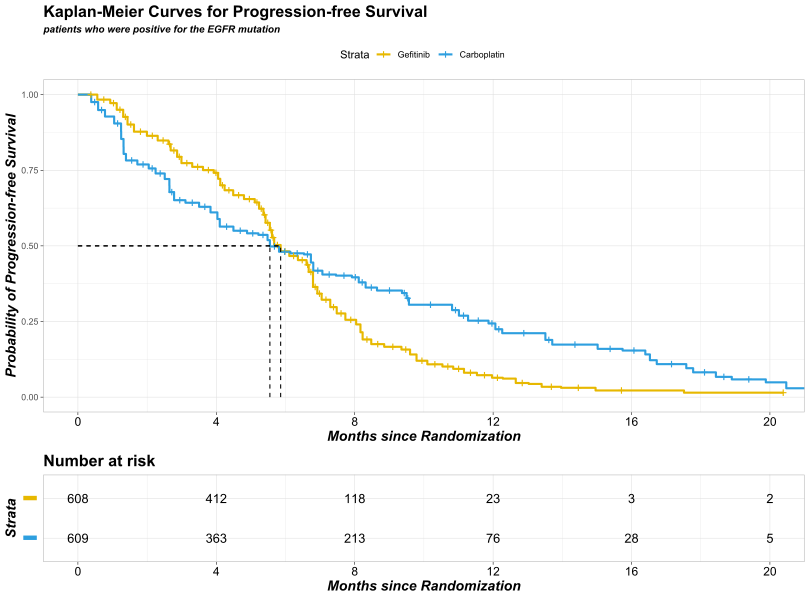
\includegraphics[scale=0.55]{figure/mok.2.a} 

}

\caption{Patients with unknown EGFR mutation status}\label{fig:unnamed-chunk-3}
\end{figure}
\clearpage

\hypertarget{brehmer-et-al.-2016-nivolumab-versus-docetaxel-study-crossing-hazards}{%
\subsubsection{Brehmer et al.~2016 Nivolumab versus Docetaxel Study: Crossing Hazards}\label{brehmer-et-al.-2016-nivolumab-versus-docetaxel-study-crossing-hazards}}
\begin{figure}

{\centering 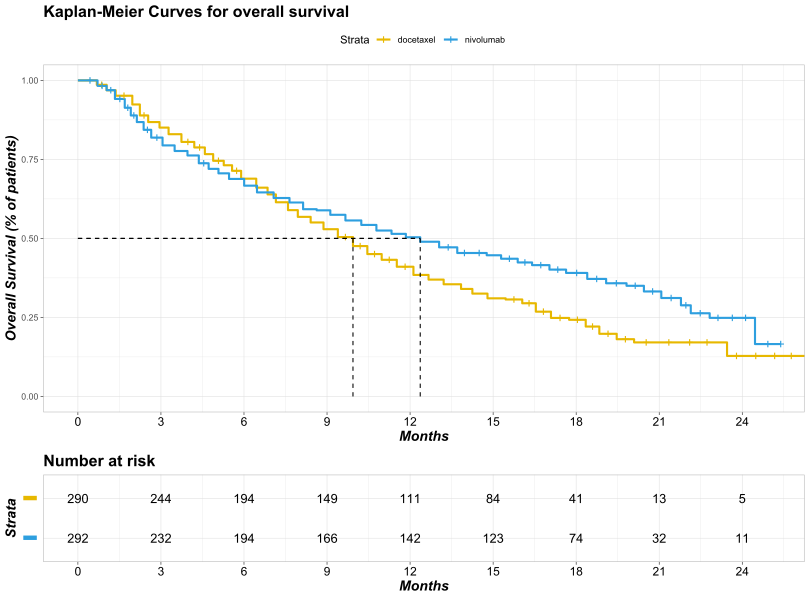
\includegraphics[scale=0.55]{figure/brehmer} 

}

\caption{Kaplan–Meier curves for overall survival}\label{fig:unnamed-chunk-5}
\end{figure}
\clearpage

\hypertarget{mok-et-al.-2009-ipass-study-dimishing-treatment-effect}{%
\subsubsection{Mok et al.~2009 IPASS Study: Dimishing Treatment Effect}\label{mok-et-al.-2009-ipass-study-dimishing-treatment-effect}}
\begin{figure}

{\centering 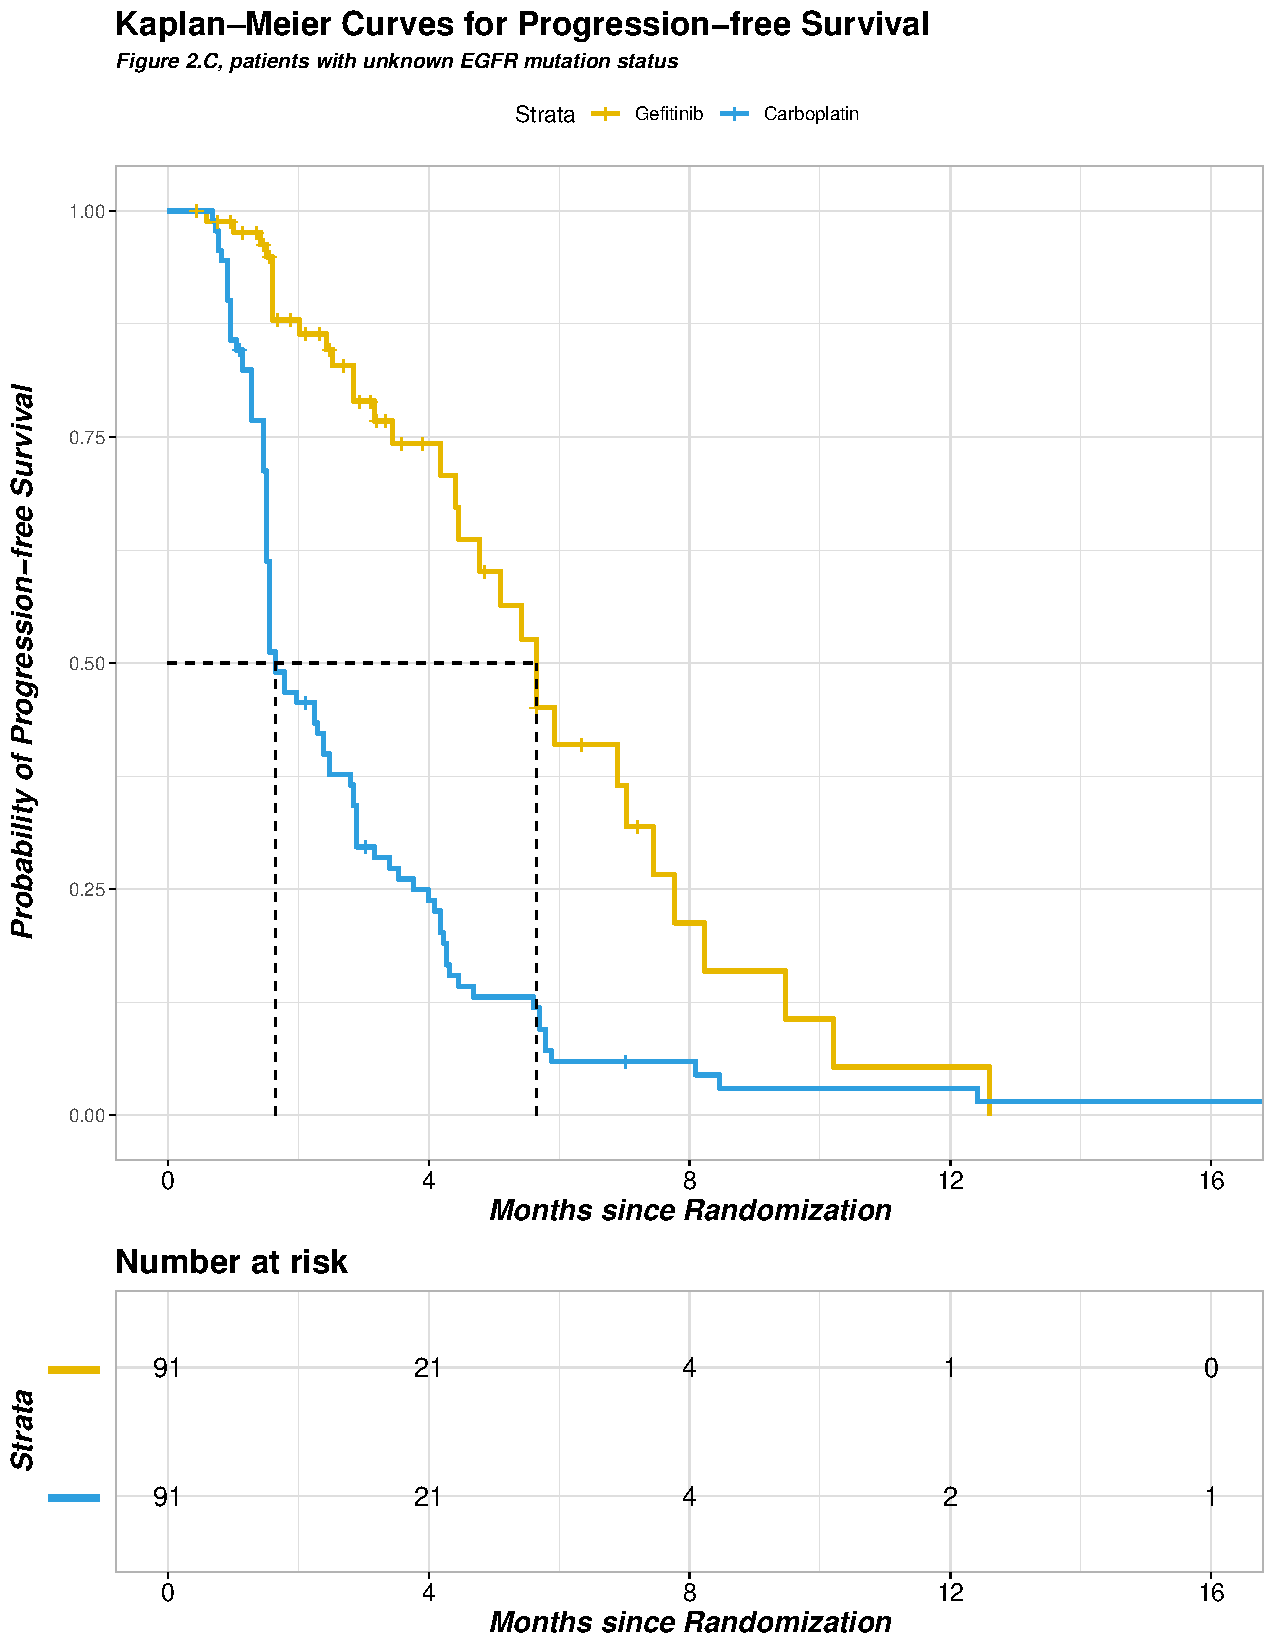
\includegraphics[scale=0.55]{figure/mok.2.c} 

}

\caption{Patients with unknown EGFR mutation status}\label{fig:unnamed-chunk-7}
\end{figure}
\clearpage

\hypertarget{ohtsu-et-al.-2011-avagast-study-dimishing-treatment-effect}{%
\subsubsection{Ohtsu et al.~2011 AVAGAST Study: Dimishing Treatment Effect}\label{ohtsu-et-al.-2011-avagast-study-dimishing-treatment-effect}}
\begin{figure}

{\centering 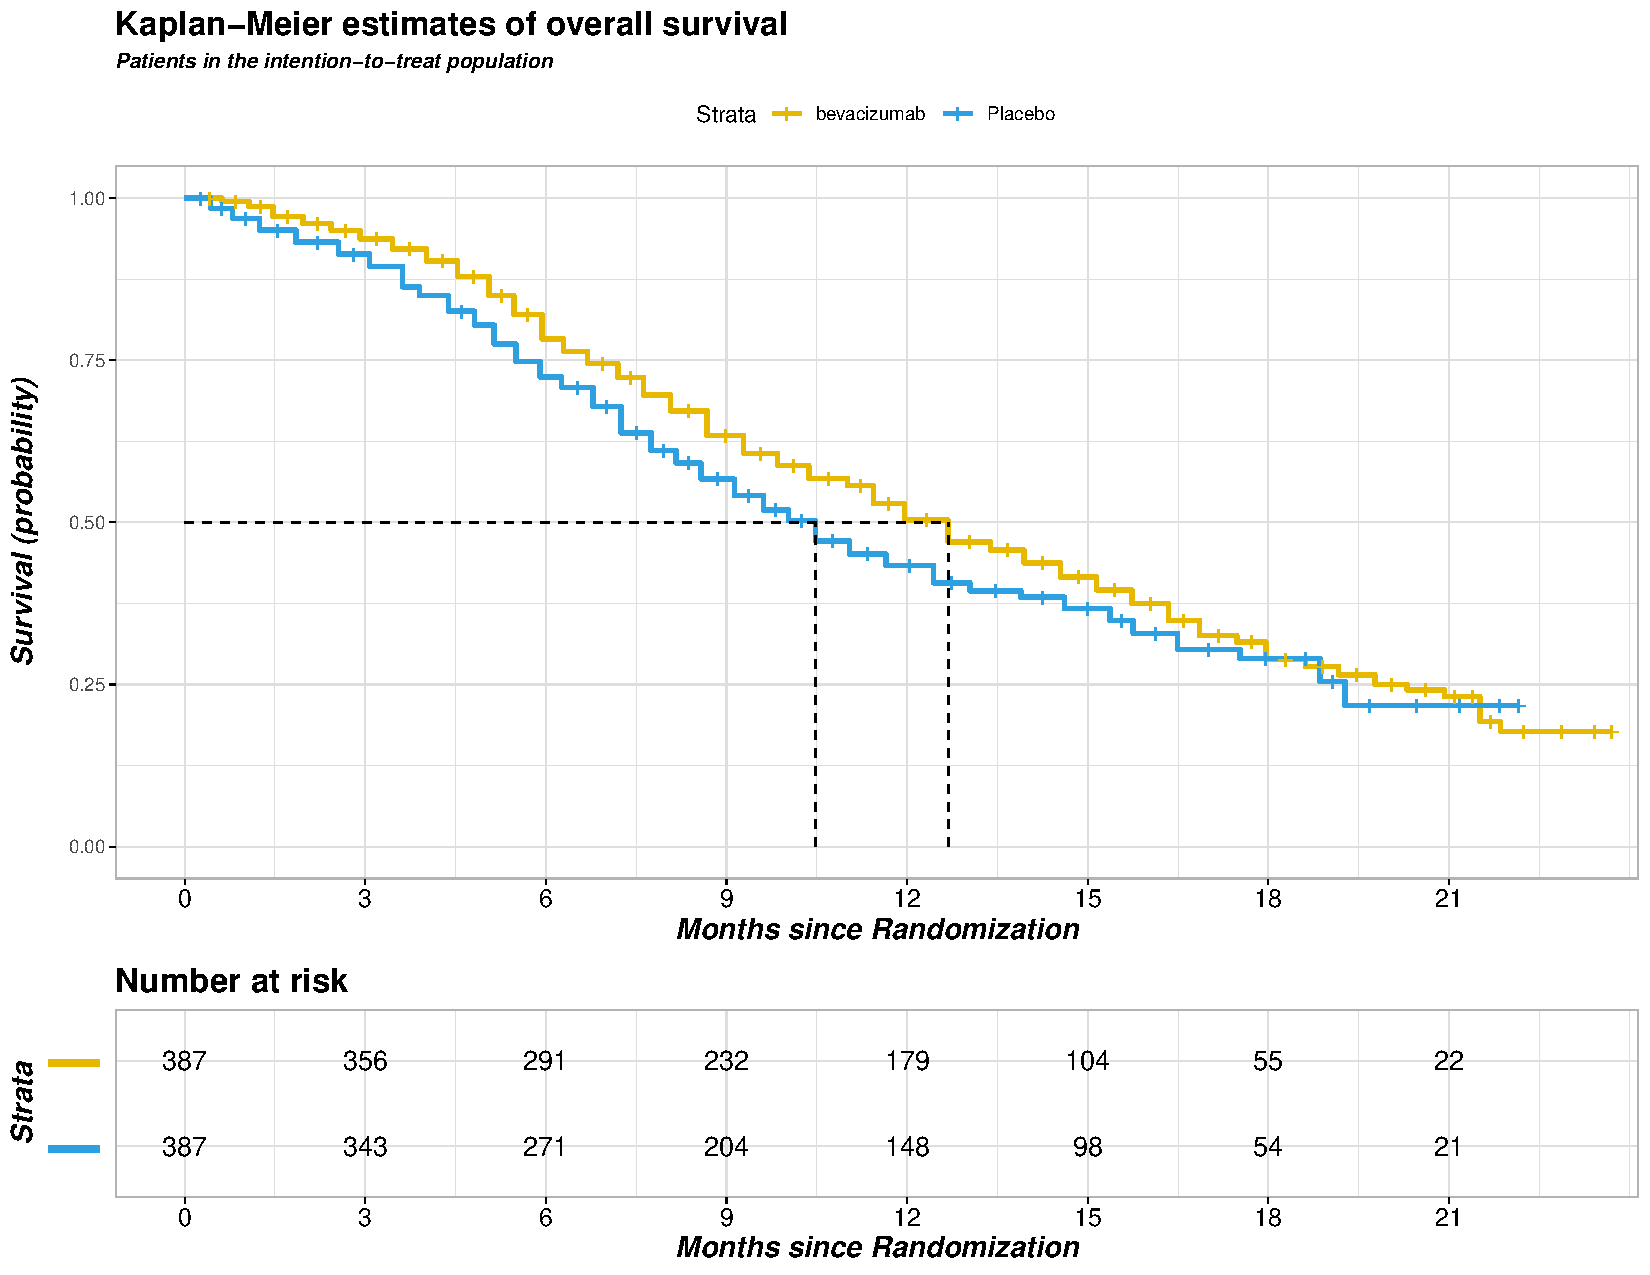
\includegraphics[scale=0.55]{figure/ohtsu} 

}

\caption{Patients in the intention-to-treat population}\label{fig:unnamed-chunk-9}
\end{figure}
\clearpage

\hypertarget{ascierto-et-al.-2017-the-ipilimumab-study-delayed-treatment-effect}{%
\subsubsection{Ascierto et al.~2017 The Ipilimumab Study: Delayed Treatment Effect}\label{ascierto-et-al.-2017-the-ipilimumab-study-delayed-treatment-effect}}
\begin{figure}

{\centering 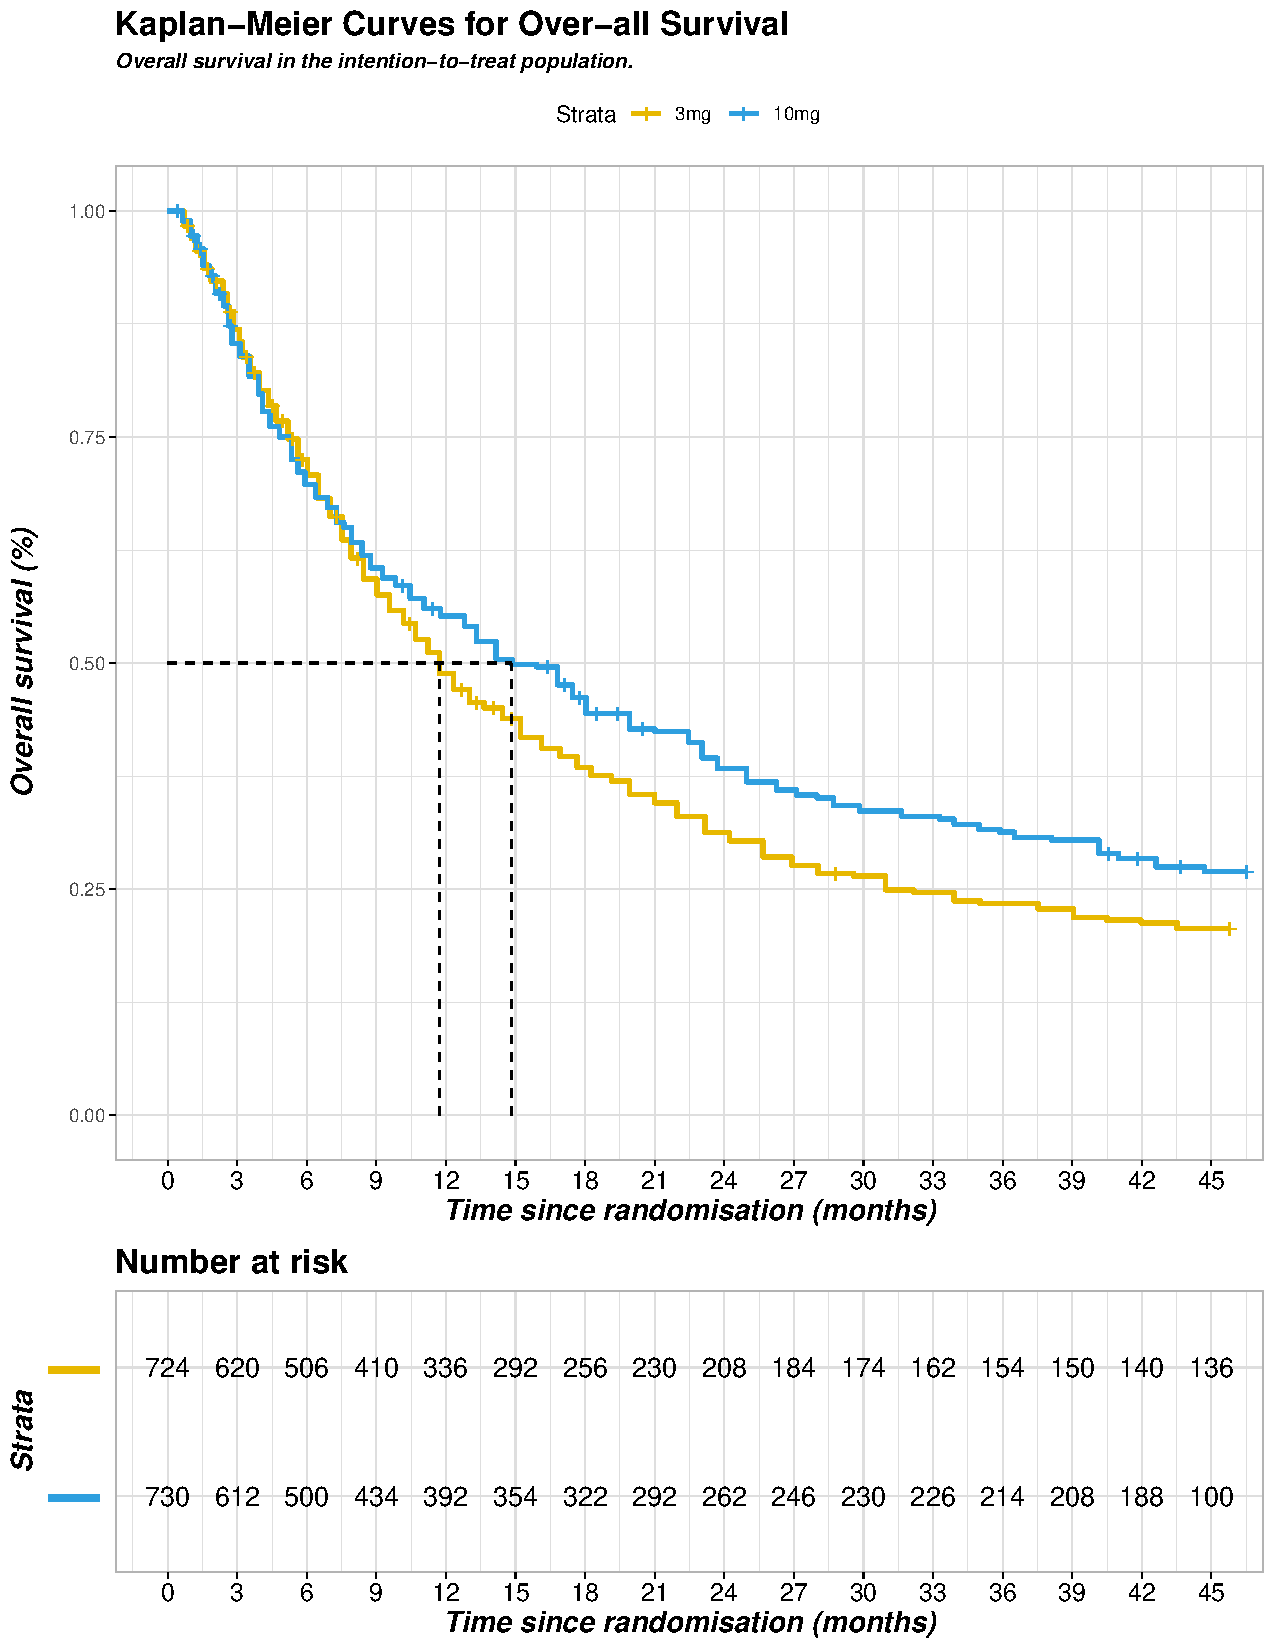
\includegraphics[scale=0.55]{figure/ascierto} 

}

\caption{Patients in the intention-to-treat population}\label{fig:unnamed-chunk-11}
\end{figure}
\clearpage

\hypertarget{reck-et-al.-2018-the-impower150-study-delayed-treatment-effect}{%
\subsubsection{Reck et al.~2018 The IMpower150 Study: Delayed Treatment Effect}\label{reck-et-al.-2018-the-impower150-study-delayed-treatment-effect}}
\begin{figure}

{\centering 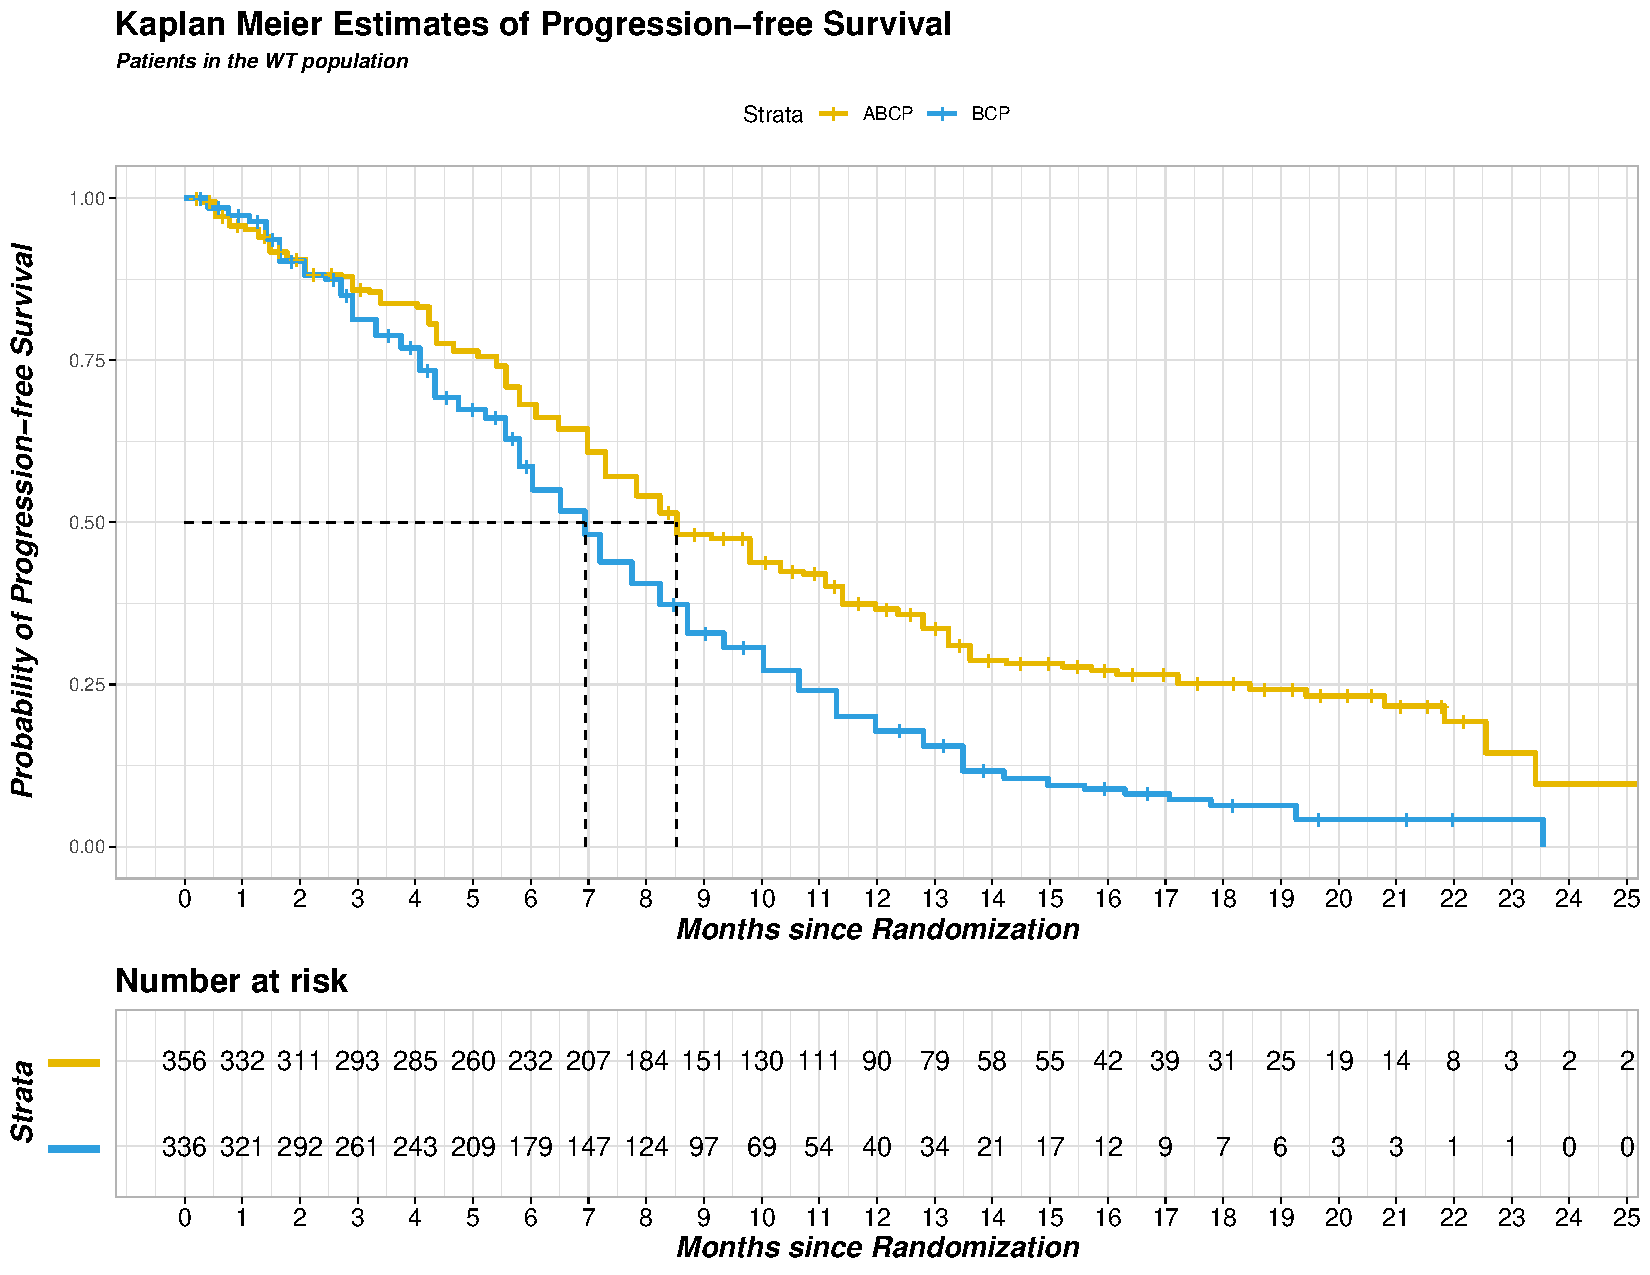
\includegraphics[scale=0.55]{figure/reck} 

}

\caption{Patients in the WT population}\label{fig:unnamed-chunk-13}
\end{figure}
\hypertarget{math}{%
\section{Math}\label{math}}

\TeX~is the best way to typeset mathematics. Donald Knuth designed \TeX~when he got frustrated at how long it was taking the typesetters to finish his book, which contained a lot of mathematics. One nice feature of \emph{R Markdown} is its ability to read LaTeX code directly.

If you are doing a thesis that will involve lots of math, you will want to read the following section which has been commented out. If you're not going to use math, skip over or delete this next commented section.

\hypertarget{chemistry-101-symbols}{%
\section{Chemistry 101: Symbols}\label{chemistry-101-symbols}}

Chemical formulas will look best if they are not italicized. Get around math mode's automatic italicizing in LaTeX by using the argument \texttt{\$\textbackslash{}mathrm\{formula\ here\}\$}, with your formula inside the curly brackets. (Notice the use of the backticks here which enclose text that acts as code.)

So, \(\mathrm{Fe_2^{2+}Cr_2O_4}\) is written \texttt{\$\textbackslash{}mathrm\{Fe\_2\^{}\{2+\}Cr\_2O\_4\}\$}.

\noindent Exponent or Superscript: \(\mathrm{O^-}\)

\noindent Subscript: \(\mathrm{CH_4}\)

To stack numbers or letters as in \(\mathrm{Fe_2^{2+}}\), the subscript is defined first, and then the superscript is defined.

\noindent Bullet: CuCl \(\bullet\) \(\mathrm{7H_{2}O}\)

\noindent Delta: \(\Delta\)

\noindent Reaction Arrows: \(\longrightarrow\) or \(\xrightarrow{solution}\)

\noindent Resonance Arrows: \(\leftrightarrow\)

\noindent Reversible Reaction Arrows: \(\rightleftharpoons\)

\hypertarget{typesetting-reactions}{%
\subsection{Typesetting reactions}\label{typesetting-reactions}}

You may wish to put your reaction in an equation environment, which means that LaTeX will place the reaction where it fits and will number the equations for you.
\begin{equation}
  \mathrm{C_6H_{12}O_6  + 6O_2} \longrightarrow \mathrm{6CO_2 + 6H_2O}
  \label{eq:reaction}
\end{equation}
We can reference this combustion of glucose reaction via Equation \eqref{eq:reaction}.

\hypertarget{other-examples-of-reactions}{%
\subsection{Other examples of reactions}\label{other-examples-of-reactions}}

\(\mathrm{NH_4Cl_{(s)}}\) \(\rightleftharpoons\) \(\mathrm{NH_{3(g)}+HCl_{(g)}}\)

\noindent \(\mathrm{MeCH_2Br + Mg}\) \(\xrightarrow[below]{above}\) \(\mathrm{MeCH_2\bullet Mg \bullet Br}\)

\hypertarget{physics}{%
\section{Physics}\label{physics}}

Many of the symbols you will need can be found on the math page \url{https://web.reed.edu/cis/help/latex/math.html} and the Comprehensive LaTeX Symbol Guide (\url{https://mirror.utexas.edu/ctan/info/symbols/comprehensive/symbols-letter.pdf}).

\hypertarget{biology}{%
\section{Biology}\label{biology}}

You will probably find the resources at \url{https://www.lecb.ncifcrf.gov/~toms/latex.html} helpful, particularly the links to bsts for various journals. You may also be interested in TeXShade for nucleotide typesetting (\url{https://homepages.uni-tuebingen.de/beitz/txe.html}). Be sure to read the proceeding chapter on graphics and tables.

\hypertarget{ref-labels}{%
\chapter{Tables, Graphics, References, and Labels}\label{ref-labels}}

\hypertarget{tables}{%
\section{Tables}\label{tables}}

In addition to the tables that can be automatically generated from a data frame in \textbf{R} that you saw in {[}R Markdown Basics{]} using the \texttt{kable()} function, you can also create tables using \emph{pandoc}. (More information is available at \url{https://pandoc.org/README.html\#tables}.) This might be useful if you don't have values specifically stored in \textbf{R}, but you'd like to display them in table form. Below is an example. Pay careful attention to the alignment in the table and hyphens to create the rows and columns.
\begin{longtable}[]{@{}ccc@{}}
\caption{\label{tab:inher} Correlation of Inheritance Factors for Parents and Child}\tabularnewline
\toprule
\begin{minipage}[b]{0.29\columnwidth}\centering
Factors\strut
\end{minipage} & \begin{minipage}[b]{0.46\columnwidth}\centering
Correlation between Parents \& Child\strut
\end{minipage} & \begin{minipage}[b]{0.16\columnwidth}\centering
Inherited\strut
\end{minipage}\tabularnewline
\midrule
\endfirsthead
\toprule
\begin{minipage}[b]{0.29\columnwidth}\centering
Factors\strut
\end{minipage} & \begin{minipage}[b]{0.46\columnwidth}\centering
Correlation between Parents \& Child\strut
\end{minipage} & \begin{minipage}[b]{0.16\columnwidth}\centering
Inherited\strut
\end{minipage}\tabularnewline
\midrule
\endhead
\begin{minipage}[t]{0.29\columnwidth}\centering
Education\strut
\end{minipage} & \begin{minipage}[t]{0.46\columnwidth}\centering
-0.49\strut
\end{minipage} & \begin{minipage}[t]{0.16\columnwidth}\centering
Yes\strut
\end{minipage}\tabularnewline
\begin{minipage}[t]{0.29\columnwidth}\centering
Socio-Economic Status\strut
\end{minipage} & \begin{minipage}[t]{0.46\columnwidth}\centering
0.28\strut
\end{minipage} & \begin{minipage}[t]{0.16\columnwidth}\centering
Slight\strut
\end{minipage}\tabularnewline
\begin{minipage}[t]{0.29\columnwidth}\centering
Income\strut
\end{minipage} & \begin{minipage}[t]{0.46\columnwidth}\centering
0.08\strut
\end{minipage} & \begin{minipage}[t]{0.16\columnwidth}\centering
No\strut
\end{minipage}\tabularnewline
\begin{minipage}[t]{0.29\columnwidth}\centering
Family Size\strut
\end{minipage} & \begin{minipage}[t]{0.46\columnwidth}\centering
0.18\strut
\end{minipage} & \begin{minipage}[t]{0.16\columnwidth}\centering
Slight\strut
\end{minipage}\tabularnewline
\begin{minipage}[t]{0.29\columnwidth}\centering
Occupational Prestige\strut
\end{minipage} & \begin{minipage}[t]{0.46\columnwidth}\centering
0.21\strut
\end{minipage} & \begin{minipage}[t]{0.16\columnwidth}\centering
Slight\strut
\end{minipage}\tabularnewline
\bottomrule
\end{longtable}
We can also create a link to the table by doing the following: Table \ref{tab:inher}. If you go back to {[}Loading and exploring data{]} and look at the \texttt{kable} table, we can create a reference to this max delays table too: Table \ref{tab:maxdelays}. The addition of the \texttt{(\textbackslash{}\#tab:inher)} option to the end of the table caption allows us to then make a reference to Table \texttt{\textbackslash{}@ref(tab:label)}. Note that this reference could appear anywhere throughout the document after the table has appeared.

\clearpage

\hypertarget{figures}{%
\section{Figures}\label{figures}}

If your thesis has a lot of figures, \emph{R Markdown} might behave better for you than that other word processor. One perk is that it will automatically number the figures accordingly in each chapter. You'll also be able to create a label for each figure, add a caption, and then reference the figure in a way similar to what we saw with tables earlier. If you label your figures, you can move the figures around and \emph{R Markdown} will automatically adjust the numbering for you. No need for you to remember! So that you don't have to get too far into LaTeX to do this, a couple \textbf{R} functions have been created for you to assist. You'll see their use below.

In the \textbf{R} chunk below, we will load in a picture stored as \texttt{reed.jpg} in our main directory. We then give it the caption of ``Reed logo'', the label of ``reedlogo'', and specify that this is a figure. Make note of the different \textbf{R} chunk options that are given in the R Markdown file (not shown in the knitted document).
\begin{Shaded}
\begin{Highlighting}[]
\KeywordTok{include_graphics}\NormalTok{(}\DataTypeTok{path =} \StringTok{"figure/reed.jpg"}\NormalTok{)}
\end{Highlighting}
\end{Shaded}
\begin{figure}

\includegraphics[width=3.47in]{figure/reed} \caption{Reed logo}\label{fig:reedlogo}
\end{figure}
Here is a reference to the Reed logo: Figure \ref{fig:reedlogo}. Note the use of the \texttt{fig:} code here. By naming the \textbf{R} chunk that contains the figure, we can then reference that figure later as done in the first sentence here. We can also specify the caption for the figure via the R chunk option \texttt{fig.cap}.

\clearpage

Below we will investigate how to save the output of an \textbf{R} plot and label it in a way similar to that done above. Recall the \texttt{flights} dataset from Chapter \ref{rmd-basics}. (Note that we've shown a different way to reference a section or chapter here.) We will next explore a bar graph with the mean flight departure delays by airline from Portland for 2014.
\begin{Shaded}
\begin{Highlighting}[]
\NormalTok{mean_delay_by_carrier <-}\StringTok{ }\NormalTok{flights }\OperatorTok
\StringTok{  }\KeywordTok{group_by}\NormalTok{(carrier) }\OperatorTok
\StringTok{  }\KeywordTok{summarize}\NormalTok{(}\DataTypeTok{mean_dep_delay =} \KeywordTok{mean}\NormalTok{(dep_delay))}
\end{Highlighting}
\end{Shaded}
\begin{verbatim}
`summarise()` ungrouping output (override with `.groups` argument)
\end{verbatim}
\begin{Shaded}
\begin{Highlighting}[]
\KeywordTok{ggplot}\NormalTok{(mean_delay_by_carrier, }\KeywordTok{aes}\NormalTok{(}\DataTypeTok{x =}\NormalTok{ carrier, }\DataTypeTok{y =}\NormalTok{ mean_dep_delay)) }\OperatorTok{+}
\StringTok{  }\KeywordTok{geom_bar}\NormalTok{(}\DataTypeTok{position =} \StringTok{"identity"}\NormalTok{, }\DataTypeTok{stat =} \StringTok{"identity"}\NormalTok{, }\DataTypeTok{fill =} \StringTok{"red"}\NormalTok{)}
\end{Highlighting}
\end{Shaded}
\begin{figure}
\centering
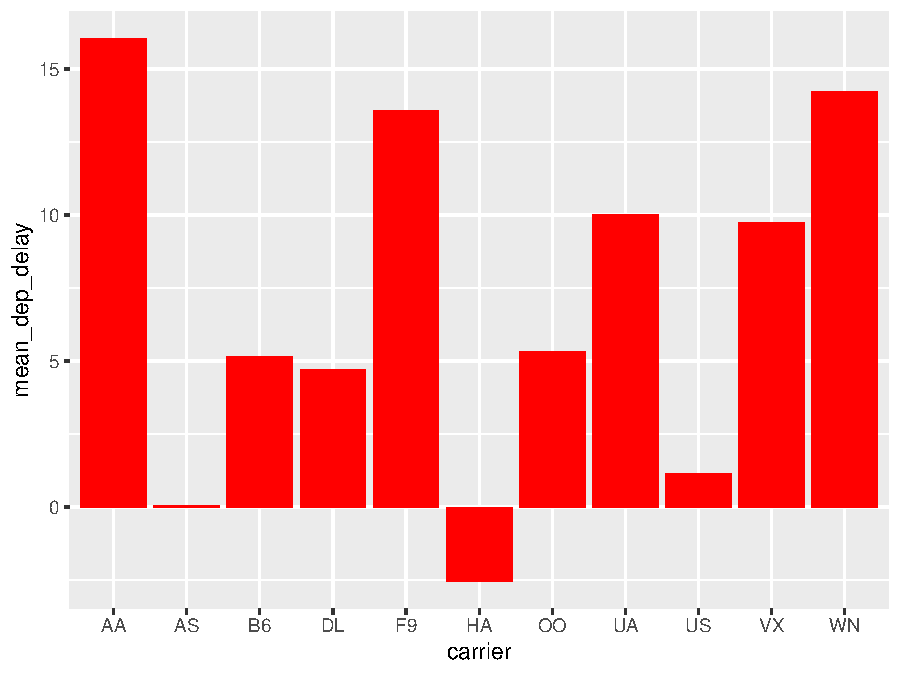
\includegraphics{thesis_files/figure-latex/delaysboxplot-1.pdf}
\caption{\label{fig:delaysboxplot}Mean Delays by Airline}
\end{figure}
Here is a reference to this image: Figure \ref{fig:delaysboxplot}.

A table linking these carrier codes to airline names is available at \url{https://github.com/ismayc/pnwflights14/blob/master/data/airlines.csv}.

\clearpage

Next, we will explore the use of the \texttt{out.extra} chunk option, which can be used to shrink or expand an image loaded from a file by specifying \texttt{"scale=\ "}. Here we use the mathematical graph stored in the ``subdivision.pdf'' file.
\begin{figure}
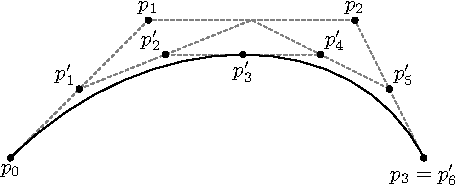
\includegraphics[scale=0.75]{figure/subdivision} \caption{Subdiv. graph}\label{fig:subd}
\end{figure}
Here is a reference to this image: Figure \ref{fig:subd}. Note that \texttt{echo=FALSE} is specified so that the \textbf{R} code is hidden in the document.

\textbf{More Figure Stuff}

Lastly, we will explore how to rotate and enlarge figures using the \texttt{out.extra} chunk option. (Currently this only works in the PDF version of the book.)
\begin{figure}
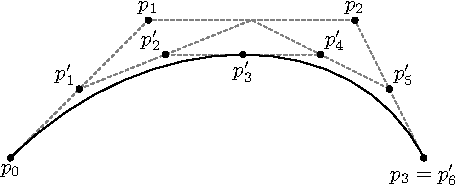
\includegraphics[angle=180, scale=1.1]{figure/subdivision} \caption{A Larger Figure, Flipped Upside Down}\label{fig:subd2}
\end{figure}
As another example, here is a reference: Figure \ref{fig:subd2}.

\hypertarget{footnotes-and-endnotes}{%
\section{Footnotes and Endnotes}\label{footnotes-and-endnotes}}

You might want to footnote something.\footnote{footnote text} The footnote will be in a smaller font and placed appropriately. Endnotes work in much the same way. More information can be found about both on the CUS site or feel free to reach out to \href{mailto:data@reed.edu}{\nolinkurl{data@reed.edu}}.

\hypertarget{bibliographies}{%
\section{Bibliographies}\label{bibliographies}}

Of course you will need to cite things, and you will probably accumulate an armful of sources. There are a variety of tools available for creating a bibliography database (stored with the .bib extension). In addition to BibTeX suggested below, you may want to consider using the free and easy-to-use tool called Zotero. The Reed librarians have created Zotero documentation at \url{https://libguides.reed.edu/citation/zotero}. In addition, a tutorial is available from Middlebury College at \url{https://sites.middlebury.edu/zoteromiddlebury/}.

\emph{R Markdown} uses \emph{pandoc} (\url{https://pandoc.org/}) to build its bibliographies. One nice caveat of this is that you won't have to do a second compile to load in references as standard LaTeX requires. To cite references in your thesis (after creating your bibliography database), place the reference name inside square brackets and precede it by the ``at'' symbol. For example, here's a reference to a book about worrying: (Molina \& Borkovec, 1994). This \texttt{Molina1994} entry appears in a file called \texttt{thesis.bib} in the \texttt{bib} folder. This bibliography database file was created by a program called BibTeX. You can call this file something else if you like (look at the YAML header in the main .Rmd file) and, by default, is to placed in the \texttt{bib} folder.

For more information about BibTeX and bibliographies, see our CUS site (\url{https://web.reed.edu/cis/help/latex/index.html})\footnote{Reed~College (2007)}. There are three pages on this topic: \emph{bibtex} (which talks about using BibTeX, at \url{https://web.reed.edu/cis/help/latex/bibtex.html}), \emph{bibtexstyles} (about how to find and use the bibliography style that best suits your needs, at \url{https://web.reed.edu/cis/help/latex/bibtexstyles.html}) and \emph{bibman} (which covers how to make and maintain a bibliography by hand, without BibTeX, at \url{https://web.reed.edu/cis/help/latex/bibman.html}). The last page will not be useful unless you have only a few sources.

If you look at the YAML header at the top of the main .Rmd file you can see that we can specify the style of the bibliography by referencing the appropriate csl file. You can download a variety of different style files at \url{https://www.zotero.org/styles}. Make sure to download the file into the csl folder.

\vfill

\textbf{Tips for Bibliographies}
\begin{itemize}
\tightlist
\item
  Like with thesis formatting, the sooner you start compiling your bibliography for something as large as thesis, the better. Typing in source after source is mind-numbing enough; do you really want to do it for hours on end in late April? Think of it as procrastination.
\item
  The cite key (a citation's label) needs to be unique from the other entries.
\item
  When you have more than one author or editor, you need to separate each author's name by the word ``and'' e.g.~\texttt{Author\ =\ \{Noble,\ Sam\ and\ Youngberg,\ Jessica\},}.
\item
  Bibliographies made using BibTeX (whether manually or using a manager) accept LaTeX markup, so you can italicize and add symbols as necessary.
\item
  To force capitalization in an article title or where all lowercase is generally used, bracket the capital letter in curly braces.
\item
  You can add a Reed Thesis citation\footnote{Noble (2002)} option. The best way to do this is to use the phdthesis type of citation, and use the optional ``type'' field to enter ``Reed thesis'' or ``Undergraduate thesis.''
\end{itemize}
\hypertarget{anything-else}{%
\section{Anything else?}\label{anything-else}}

If you'd like to see examples of other things in this template, please contact the Data @ Reed team (email \href{mailto:data@reed.edu}{\nolinkurl{data@reed.edu}}) with your suggestions. We love to see people using \emph{R Markdown} for their theses, and are happy to help.

\hypertarget{conclusion}{%
\chapter*{Conclusion}\label{conclusion}}
\addcontentsline{toc}{chapter}{Conclusion}

If we don't want Conclusion to have a chapter number next to it, we can add the \texttt{\{-\}} attribute.

\textbf{More info}

And here's some other random info: the first paragraph after a chapter title or section head \emph{shouldn't be} indented, because indents are to tell the reader that you're starting a new paragraph. Since that's obvious after a chapter or section title, proper typesetting doesn't add an indent there.

\appendix

\hypertarget{the-first-appendix}{%
\chapter{The First Appendix}\label{the-first-appendix}}

This first appendix includes all of the R chunks of code that were hidden throughout the document (using the \texttt{include\ =\ FALSE} chunk tag) to help with readibility and/or setup.

\textbf{In the main Rmd file}
\begin{Shaded}
\begin{Highlighting}[]
\CommentTok{# This chunk ensures that the thesisdown package is}
\CommentTok{# installed and loaded. This thesisdown package includes}
\CommentTok{# the template files for the thesis.}
\ControlFlowTok{if}\NormalTok{ (}\OperatorTok{!}\KeywordTok{require}\NormalTok{(remotes)) \{}
  \ControlFlowTok{if}\NormalTok{ (params}\OperatorTok{$}\StringTok{`}\DataTypeTok{Install needed packages for \{thesisdown\}}\StringTok{`}\NormalTok{) \{}
    \KeywordTok{install.packages}\NormalTok{(}\StringTok{"remotes"}\NormalTok{, }\DataTypeTok{repos =} \StringTok{"https://cran.rstudio.com"}\NormalTok{)}
\NormalTok{  \} }\ControlFlowTok{else}\NormalTok{ \{}
    \KeywordTok{stop}\NormalTok{(}
      \KeywordTok{paste}\NormalTok{(}\StringTok{'You need to run install.packages("remotes")",}
\StringTok{            "first in the Console.'}\NormalTok{)}
\NormalTok{    )}
\NormalTok{  \}}
\NormalTok{\}}
\ControlFlowTok{if}\NormalTok{ (}\OperatorTok{!}\KeywordTok{require}\NormalTok{(thesisdown)) \{}
  \ControlFlowTok{if}\NormalTok{ (params}\OperatorTok{$}\StringTok{`}\DataTypeTok{Install needed packages for \{thesisdown\}}\StringTok{`}\NormalTok{) \{}
\NormalTok{    remotes}\OperatorTok{::}\KeywordTok{install_github}\NormalTok{(}\StringTok{"ismayc/thesisdown"}\NormalTok{)}
\NormalTok{  \} }\ControlFlowTok{else}\NormalTok{ \{}
    \KeywordTok{stop}\NormalTok{(}
      \KeywordTok{paste}\NormalTok{(}
        \StringTok{"You need to run"}\NormalTok{,}
        \StringTok{'remotes::install_github("ismayc/thesisdown")'}\NormalTok{,}
        \StringTok{"first in the Console."}
\NormalTok{      )}
\NormalTok{    )}
\NormalTok{  \}}
\NormalTok{\}}
\KeywordTok{library}\NormalTok{(thesisdown)}
\CommentTok{# Set how wide the R output will go}
\KeywordTok{options}\NormalTok{(}\DataTypeTok{width =} \DecValTok{70}\NormalTok{)}
\end{Highlighting}
\end{Shaded}
\textbf{In Chapter \ref{ref-labels}:}
\begin{Shaded}
\begin{Highlighting}[]
\CommentTok{# This chunk ensures that the thesisdown package is}
\CommentTok{# installed and loaded. This thesisdown package includes}
\CommentTok{# the template files for the thesis and also two functions}
\CommentTok{# used for labeling and referencing}
\ControlFlowTok{if}\NormalTok{ (}\OperatorTok{!}\KeywordTok{require}\NormalTok{(remotes)) \{}
  \ControlFlowTok{if}\NormalTok{ (params}\OperatorTok{$}\StringTok{`}\DataTypeTok{Install needed packages for \{thesisdown\}}\StringTok{`}\NormalTok{) \{}
    \KeywordTok{install.packages}\NormalTok{(}\StringTok{"remotes"}\NormalTok{, }\DataTypeTok{repos =} \StringTok{"https://cran.rstudio.com"}\NormalTok{)}
\NormalTok{  \} }\ControlFlowTok{else}\NormalTok{ \{}
    \KeywordTok{stop}\NormalTok{(}
      \KeywordTok{paste}\NormalTok{(}
        \StringTok{'You need to run install.packages("remotes")'}\NormalTok{,}
        \StringTok{"first in the Console."}
\NormalTok{      )}
\NormalTok{    )}
\NormalTok{  \}}
\NormalTok{\}}
\ControlFlowTok{if}\NormalTok{ (}\OperatorTok{!}\KeywordTok{require}\NormalTok{(dplyr)) \{}
  \ControlFlowTok{if}\NormalTok{ (params}\OperatorTok{$}\StringTok{`}\DataTypeTok{Install needed packages for \{thesisdown\}}\StringTok{`}\NormalTok{) \{}
    \KeywordTok{install.packages}\NormalTok{(}\StringTok{"dplyr"}\NormalTok{, }\DataTypeTok{repos =} \StringTok{"https://cran.rstudio.com"}\NormalTok{)}
\NormalTok{  \} }\ControlFlowTok{else}\NormalTok{ \{}
    \KeywordTok{stop}\NormalTok{(}
      \KeywordTok{paste}\NormalTok{(}
        \StringTok{'You need to run install.packages("dplyr")'}\NormalTok{,}
        \StringTok{"first in the Console."}
\NormalTok{      )}
\NormalTok{    )}
\NormalTok{  \}}
\NormalTok{\}}
\ControlFlowTok{if}\NormalTok{ (}\OperatorTok{!}\KeywordTok{require}\NormalTok{(ggplot2)) \{}
  \ControlFlowTok{if}\NormalTok{ (params}\OperatorTok{$}\StringTok{`}\DataTypeTok{Install needed packages for \{thesisdown\}}\StringTok{`}\NormalTok{) \{}
    \KeywordTok{install.packages}\NormalTok{(}\StringTok{"ggplot2"}\NormalTok{, }\DataTypeTok{repos =} \StringTok{"https://cran.rstudio.com"}\NormalTok{)}
\NormalTok{  \} }\ControlFlowTok{else}\NormalTok{ \{}
    \KeywordTok{stop}\NormalTok{(}
      \KeywordTok{paste}\NormalTok{(}
        \StringTok{'You need to run install.packages("ggplot2")'}\NormalTok{,}
        \StringTok{"first in the Console."}
\NormalTok{      )}
\NormalTok{    )}
\NormalTok{  \}}
\NormalTok{\}}
\ControlFlowTok{if}\NormalTok{ (}\OperatorTok{!}\KeywordTok{require}\NormalTok{(bookdown)) \{}
  \ControlFlowTok{if}\NormalTok{ (params}\OperatorTok{$}\StringTok{`}\DataTypeTok{Install needed packages for \{thesisdown\}}\StringTok{`}\NormalTok{) \{}
    \KeywordTok{install.packages}\NormalTok{(}\StringTok{"bookdown"}\NormalTok{, }\DataTypeTok{repos =} \StringTok{"https://cran.rstudio.com"}\NormalTok{)}
\NormalTok{  \} }\ControlFlowTok{else}\NormalTok{ \{}
    \KeywordTok{stop}\NormalTok{(}
      \KeywordTok{paste}\NormalTok{(}
        \StringTok{'You need to run install.packages("bookdown")'}\NormalTok{,}
        \StringTok{"first in the Console."}
\NormalTok{      )}
\NormalTok{    )}
\NormalTok{  \}}
\NormalTok{\}}
\ControlFlowTok{if}\NormalTok{ (}\OperatorTok{!}\KeywordTok{require}\NormalTok{(thesisdown)) \{}
  \ControlFlowTok{if}\NormalTok{ (params}\OperatorTok{$}\StringTok{`}\DataTypeTok{Install needed packages for \{thesisdown\}}\StringTok{`}\NormalTok{) \{}
\NormalTok{    remotes}\OperatorTok{::}\KeywordTok{install_github}\NormalTok{(}\StringTok{"ismayc/thesisdown"}\NormalTok{)}
\NormalTok{  \} }\ControlFlowTok{else}\NormalTok{ \{}
    \KeywordTok{stop}\NormalTok{(}
      \KeywordTok{paste}\NormalTok{(}
        \StringTok{"You need to run"}\NormalTok{,}
        \StringTok{'remotes::install_github("ismayc/thesisdown")'}\NormalTok{,}
        \StringTok{"first in the Console."}
\NormalTok{      )}
\NormalTok{    )}
\NormalTok{  \}}
\NormalTok{\}}
\KeywordTok{library}\NormalTok{(thesisdown)}
\KeywordTok{library}\NormalTok{(dplyr)}
\KeywordTok{library}\NormalTok{(ggplot2)}
\KeywordTok{library}\NormalTok{(knitr)}
\NormalTok{flights <-}\StringTok{ }\KeywordTok{read.csv}\NormalTok{(}\StringTok{"data/flights.csv"}\NormalTok{, }\DataTypeTok{stringsAsFactors =} \OtherTok{FALSE}\NormalTok{)}
\end{Highlighting}
\end{Shaded}
\hypertarget{the-second-appendix-for-fun}{%
\chapter{The Second Appendix, for Fun}\label{the-second-appendix-for-fun}}

\backmatter

\hypertarget{references}{%
\chapter*{References}\label{references}}
\addcontentsline{toc}{chapter}{References}

\markboth{References}{References}

\noindent

\setlength{\parindent}{-0.20in}
\setlength{\leftskip}{0.20in}
\setlength{\parskip}{8pt}

\hypertarget{refs}{}
\leavevmode\hypertarget{ref-angel2000}{}%
Angel, E. (2000). \emph{Interactive computer graphics : A top-down approach with opengl}. Boston, MA: Addison Wesley Longman.

\leavevmode\hypertarget{ref-angel2001}{}%
Angel, E. (2001a). \emph{Batch-file computer graphics : A bottom-up approach with quicktime}. Boston, MA: Wesley Addison Longman.

\leavevmode\hypertarget{ref-angel2002a}{}%
Angel, E. (2001b). \emph{Test second book by angel}. Boston, MA: Wesley Addison Longman.

\leavevmode\hypertarget{ref-Molina1994}{}%
Molina, S. T., \& Borkovec, T. D. (1994). The Penn State worry questionnaire: Psychometric properties and associated characteristics. In G. C. L. Davey \& F. Tallis (Eds.), \emph{Worrying: Perspectives on theory, assessment and treatment} (pp. 265--283). New York: Wiley.

\leavevmode\hypertarget{ref-noble2002}{}%
Noble, S. G. (2002). \emph{Turning images into simple line-art} (Undergraduate thesis). Reed College.

\leavevmode\hypertarget{ref-reedweb2007}{}%
Reed~College. (2007). LaTeX your document. Retrieved from \url{https://web.reed.edu/cis/help/LaTeX/index.html}


% Index?

\end{document}
